\section*{Discussions and Limitations}
\paragraph{sCT is less effective than sCD in latent spaces.}
As listed in \Cref{tab:cifar_in64,tab:in512}, sCT consistently outperforms sCD on CIFAR-10 and ImageNet 64$\times$64 but is less effective than sCD across different model scales on ImageNet 512$\times$512. We believe the higher training variance of CT is the main issue, particularly in the complex latent spaces defined by the pretrained encoder. We hypothesize that the current encoder/decoder may not be optimal for consistency models. Theoretically, since the ground truth mapping in consistency models aims to transform a Gaussian distribution into a multimodal data distribution with potentially disconnected supports, its tangent can become ill-conditioned at boundary points, resulting in worse optimization dynamics. If we could develop a better encoder/decoder to create a more well-conditioned ground truth mapping in the latent space, the training of consistency models would likely become significantly easier.

\paragraph{Computation costs of sCM. }
As Jacobian-vector product can be efficiently computed using \textit{forward-mode automatic differentiation}, which requires the same memory and compute as a standard forward pass without saving intermediate activations. This is significantly cheaper than backpropagation, which relies on reverse-mode automatic differentiation. Consequently, our continuous-time consistency models require similar compute and memory to train when compared to their discrete-time counterparts, which perform two forward passes at each iteration.

\paragraph{Limitations.}
Despite large improvements in FID scores, our method can still produce images with noticeable artifacts. These artifacts are commonly observed when training generative models on the ImageNet dataset with class labels, whereas training on larger datasets with caption conditions may significantly alleviate this issue. Furthermore, our 
2-step sCM still shows a small gap compared to state-of-the-art diffusion models, which we believe may be further reduced by incorporating our proposed techniques into multi-step consistency models~\citep{heek2024multistepcm}. Additionally, since FID scores do not capture all semantic details, further validation is needed to determine whether our method can scale effectively to image or video generation tasks that require larger resolutions and fine details. Besides, ensuring the training stability of sCM requires several significant modifications of the network architecture, thus sCM may be not suitable for some architectures designed for diffusion models. Moreover, our best performing method sCD still highly relies on the performance of a pretrained diffusion models, which restricts the architecture family and potentially limits the few-step generation performance. Addressing these quality issues might require new sampling strategies or enhanced architectures to maintain high fidelity even with limited sampling steps.




\section*{Appendix}
We include additional derivations, experimental details, and results in the appendix. The detailed training algorithm for sCM, covering both sCT and sCD, is provided in \Cref{appendix:algorithm}. We present a comprehensive discussion of the TrigFlow framework in \Cref{appendix:trigflow}, including detailed derivations (\Cref{appendix:trigflow_derivation}) and its connections with other parameterization (\Cref{appendix:relation_with_other_parameterization}). We introduce a new algorithm called \textit{adaptive variational score distillation} in \Cref{appendix:vsd}, which eliminates the need for manually designed training weighting. Furthermore, we elaborate on a general framework for adaptive training weighting in \Cref{appendix:adaptive_weighting}, applicable to diffusion models, consistency models, and variational score distillation. As our improvements discussed in Sec.~\ref{sec:stabilizing} are also applicable for discrete-time consistency models, we provide detailed derivations and the training algorithm for discrete-time consistency models in \Cref{appendix:discrete-trigflow}, incorporating all the improved techniques of sCM. We also provide a complete description of the Jacobian-vector product algorithm for Flash Attention in \Cref{appendix:flash_attn_jvp}. Finally, all experimental settings and evaluation results are listed in \Cref{appendix:exp}, along with additional samples generated by our sCD-XXL model trained on ImageNet at 512×512 resolution in \Cref{appendix:samples}.

\section{Training Algorithm of sCM}
\label{appendix:algorithm}

We provide the detailed algorithm of sCM in \Cref{alg:sCM}, where we refer to consistency training of sCM as \textbf{sCT} and consistency distillation of sCM as \textbf{sCD}.

\begin{algorithm}[ht]
\caption{Simplified and Stabilized Continuous-time Consistency Models (sCM).}\label{alg:sCM}
\centering
\begin{algorithmic}
\State \textbf{Input:} dataset $\gD$ with std. $\sigma_d$, pretrained diffusion model $\F_{\text{pretrain}}$ with parameter $\theta_{\text{pretrain}}$, model $\F_\theta$, weighting $w_\phi$, learning rate $\eta$, proposal ($P_{\text{mean}}, P_{\text{std}}$), constant $c$, warmup iteration $H$.
\State \textbf{Init:} $\theta \gets \theta_{\text{pretrain}}$, $\text{Iters}\gets 0$.
\Repeat
    \State $\x_0\sim \gD$, $\z\sim \gN(\vzero,\sigma_d^2\mI)$, $\tau \sim \gN(P_{\text{mean}}, P^2_{\text{std}})$, $t \gets \arctan(\frac{e^\tau}{\sigma_d})$, $\x_t \gets \cos(t)\x_0 + \sin(t)\z$
    \State $\frac{\dm \x_t}{\dm t} \gets \cos(t)\z - \sin(t)\x_0$ if consistency training else $\frac{\dm \x_t}{\dm t} \gets \sigma_d\F_{\text{pretrain}}(\frac{\x_t}{\sigma_d},t)$
    \State $r \gets \min(1, \text{Iters} / H)$ \Comment{Tangent warmup}
    \State $\vg \gets -\cos^2(t)(\sigma_d\F_{\theta^-} - \frac{\dm\x_t}{\dm t}) - r\cdot \cos(t)\sin(t) (\x_t + \sigma_d \frac{\dm \F_{\theta^-}}{\dm t})$  \Comment{JVP rearrangement}
    \State $\vg \gets \vg / (\|\vg\| + c)$ \Comment{Tangent normalization}
    \State $\gL(\theta,\phi) \gets \frac{e^{w_\phi(t)}}{D}\|
        \F_\theta(\frac{\x_t}{\sigma_d},t) - \F_{\theta^-}(\frac{\x_t}{\sigma_d},t)
        - \vg
    \|_2^2 - w_\phi(t)$ \Comment{Adaptive weighting}
    \State $(\theta, \phi) \gets (\theta, \phi) - \eta \nabla_{\theta,\phi}\gL(\theta,\phi)$
    \State $\text{Iters}\gets \text{Iters} + 1$
\Until convergence
\end{algorithmic}
\end{algorithm}


\section{TrigFlow: A Simple Framework Unifying EDM, Flow Matching and Velocity Prediction}
\label{appendix:trigflow}

\subsection{Derivations}
\label{appendix:trigflow_derivation}

Denote the standard deviation of the data distribution $p_{d}$ as $\sigma_d$. We consider a general forward diffusion process at time $t\in[0, T]$ with $\x_t = \alpha_t \x_0 + \sigma_t \z$ for the data sample $\x_0\sim p_d$ and the noise sample $\z \sim \gN(\vzero, \sigma_d^2 \mI)$ (note that the variance of $\z$ is the same as that of the data $\x_0$)\footnote{For any diffusion process with $\x_t = \alpha'_t \x_0 + \sigma'_t \vepsilon$ where $\vepsilon\sim \gN(\vzero, \mI)$, we can always equivalently convert it to $\x_t = \alpha'_t \x_0 + \frac{\sigma'_t}{\sigma_d} \cdot (\sigma_d \vepsilon)$ and let $\z \coloneqq \sigma_d \vepsilon, \alpha_t \coloneqq \alpha'_t,\sigma_t \coloneqq \frac{\sigma'_t}{\sigma_d}$. So the assumption for $\z \sim \gN(\vzero, \sigma_d^2 \mI)$ does not result in any loss of generality.}, where $\alpha_t>0,\sigma_t>0$ are \textit{noise schedules} such that $\alpha_t/\sigma_t$ is monotonically decreasing w.r.t. $t$, with $\alpha_0=1, \sigma_0=0$. The general training loss for diffusion model can always be rewritten as
\begin{equation}
    \gL_{\text{Diff}}(\theta) = \E_{\x_0,\z,t}\left[
        w(t) \left\| \D_\theta(\x_t,t) - \x_0 \right\|_2^2
    \right],
\end{equation}
where different diffusion model formulation contains four different parts:
\begin{enumerate}
    \item Parameterization of $\D_\theta$, such as score function~\citep{song2019generative,song2020score}, noise prediction model~\citep{song2019generative,song2020score,ho2020ddpm}, data prediction model~\citep{ho2020ddpm,kingma2021vdm,salimans2022progressive}, velocity prediction model~\citep{salimans2022progressive}, EDM~\citep{karras2022edm} and flow matching~\citep{lipman2022flowmatching,rectified_flow,albergo2023stochastic_interpolants}.
    \item Noise schedule for $\alpha_t$ and $\sigma_t$, such as variance preserving process~\citep{ho2020ddpm,song2020score}, variance exploding process~\citep{song2020score,karras2022edm}, cosine schedule~\citep{nichol2021improved}, and conditional optimal transport path~\citep{lipman2022flowmatching}.
    \item Weighting function for $w(t)$, such as uniform weighting~\citep{ho2020ddpm,nichol2021improved,karras2022edm}, weighting by functions of signal-to-noise-ratio (SNR)~\citep{salimans2022progressive}, monotonic weighting~\citep{kingma2024diffusion_elbo} and adaptive weighting~\citep{karras2024edm2}.
    \item Proposal distribution for $t$, such as uniform distribution within $[0, T]$~\citep{ho2020ddpm,song2020score}, log-normal distribution~\citep{karras2022edm}, SNR sampler~\citep{esser2024sd3}, and adaptive importance sampler~\citep{song2021maximum,kingma2021vdm}.
\end{enumerate}

Below we show that, under the \textit{unit variance principle} proposed in EDM~\citep{karras2022edm}, we can obtain a general but simple framework for all the above four parts, which can equivalently reproduce all previous diffusion models.

\paragraph{Step 1: General EDM parameterization.} We consider the parameterization for $\D_\theta$ as the same principle in EDM~\citep{karras2022edm} by
\begin{equation}
    \D_\theta(\x_t,t) = \cskip(t)\x_t + \cout(t) \F_\theta(\cin(t)\x_t, \cnoise(t)),
\end{equation}
and thus the training objective becomes
\begin{equation}
    \gL_{\text{Diff}} = \E_{\x_0,\z,t}\left[
        w(t)\cout^2(t) \left\| \F_\theta(\cin(t)\x_t,\cnoise(t))
        - \frac{(1-\cskip(t)\alpha_t) \x_0 - \cskip(t)\sigma_t\z}{\cout(t)}
        \right\|_2^2
    \right].
\end{equation}
To ensure the input data of $\F_\theta$ has unit variance, we should ensure $\Var[\cin(t)\x_t] = 1$ by letting
\begin{equation}
    \cin(t) = \frac{1}{\sigma_d \sqrt{\alpha_t^2 + \sigma_t^2}}.
\end{equation}
To ensure the training target of $\F_\theta$ has unit variance, we have
\begin{equation}
    \cout^2(t) = \sigma_d^2 (1 - \cskip(t)\alpha_t)^2 + \sigma_d^2\cskip^2(t)\sigma_t^2.
\end{equation}
To reduce the error amplification from $\F_\theta$ to $\D_\theta$, we should ensure $\cout(t)$ to be as small as possible, which means we should take $\cskip(t)$ by letting $\frac{\partial \cout}{\partial \cskip} = 0$, which results in
\begin{equation}
\begin{split}
    \cskip(t) = \frac{\alpha_t}{\alpha_t^2 + \sigma_t^2},\quad \cout(t) = \pm\frac{\sigma_d\sigma_t}{\sqrt{\alpha_t^2 + \sigma_t^2}}.
\end{split}
\end{equation}
Though equivalent, we choose $\cout(t) = -\frac{\sigma_d\sigma_t}{\sqrt{\alpha_t^2 + \sigma_t^2}}$ which can simplify some derivations below.

In summary, the parameterization and objective for the general diffusion noise schedule are
\begin{align}
    \D_\theta(\x_t,t) &= \frac{\alpha_t}{\alpha_t^2 + \sigma_t^2}\x_t - \frac{\sigma_t}{\sqrt{\alpha_t^2 + \sigma_t^2}} \sigma_d\F_\theta\left(\frac{\x_t}{\sigma_d \sqrt{\alpha_t^2 + \sigma_t^2}}, \cnoise(t)\right), \\
    \gL_{\text{Diff}} &= \E_{\x_0,\z,t}\left[
        w(t) \frac{\sigma^2_t}{\alpha_t^2 + \sigma_t^2}
        \left\| \sigma_d \F_\theta\left(\frac{\x_t}{\sigma_d \sqrt{\alpha_t^2 + \sigma_t^2}}, \cnoise(t)\right)
        - \frac{\alpha_t \z - \sigma_t \x_0}{\sqrt{\alpha_t^2 + \sigma_t^2}}
        \right\|_2^2
    \right].
\end{align}

\paragraph{Step 2: All noise schedules can be equivalently transformed.} One nice property of the \textit{unit variance principle} is that the $\alpha_t, \sigma_t$ in both the parameterization and the objective are \textit{homogenous}, which means we can always assume $\alpha_t^2 + \sigma_t^2 = 1$ without loss of generality. To see this, we can apply a simple change-of-variable of $\hat{\alpha}_t = \frac{\alpha_t}{\sqrt{\alpha_t^2 + \sigma_t^2}}$, $\hat{\sigma}_t = \frac{\sigma_t}{\sqrt{\alpha_t^2 + \sigma_t^2}}$ and $\hat{\x}_t = \frac{\x_t}{\sqrt{\alpha_t^2+\sigma_t^2}}=\hat{\alpha}_t \x_0 + \hat{\sigma}_t \z$, thus we have
\begin{align}
    \D_\theta(\x_t,t) &= \hat{\alpha}_t \hat{\x}_t - \hat{\sigma}_t \sigma_d \F_\theta\left(\frac{\hat{\x}_t}{\sigma_d }, \cnoise(t)\right), \\
    \gL_{\text{Diff}} &= \E_{\x_0,\z,t}\left[
        w(t) \hat{\sigma}_t^2
        \left\| \sigma_d \F_\theta\left(\frac{\hat{\x}_t}{\sigma_d}, \cnoise(t)\right)
        - (\hat{\alpha}_t \z - \hat{\sigma}_t \x_0)
        \right\|_2^2 \label{eq:appendix:trigflow:objective_general}
    \right].
\end{align}
As for the sampling procedure, according to DPM-Solver++~\citep{lu2022dpm++}, the exact solution of diffusion ODE from time $s$ to time $t$ satisfies
\begin{equation}
    \x_t = \frac{\sigma_t}{\sigma_s}\x_s + \sigma_t \int_{\lambda_s}^{\lambda_t}e^\lambda \D_\theta(\x_\lambda, \lambda)\dm\lambda,
\end{equation}
where $\lambda_t = \log\frac{\alpha_t}{\sigma_t}$, so the sampling procedure is also \textit{homogenous} for $\alpha_t,\sigma_t$. To see this, we can use the fact that $\frac{\x_t}{\sigma_t}  = \frac{\hat{\x}_t}{\hat{\sigma}_t}$ and $\lambda_t = \log \frac{\hat{\alpha}_t}{\hat{\sigma}_t} 
\coloneqq \hat{\lambda}_t$, thus the above equation is equivalent to
\begin{equation}
    \hat{\x}_t = \frac{\hat{\sigma}_t}{\hat{\sigma}_s}\hat{\x}_s + \hat{\sigma}_t \int_{\hat{\lambda}_s}^{\hat{\lambda}_t}e^{\hat{\lambda}} \hat{\D}_\theta(\hat{\x}_{\hat{\lambda}}, \hat{\lambda})\dm\hat{\lambda},
\end{equation}
which is exactly the sampling procedure of the diffusion process $\hat{\x_t}$, which means \textbf{noise schedules of diffusion models won't affect the performance of sampling}. In other words, for any diffusion process $(\alpha_t, \sigma_t, \x_t)$ at time $t$, we can always divide them by $\sqrt{\alpha_t^2 + \sigma_t^2}$ to obtain the diffusion process $(\hat{\alpha}_t, \hat{\sigma}_t, \hat{\x}_t)$ with $\hat{\alpha}_t^2 + \hat{\sigma}_t^2 = 1$ and all the parameterization, training objective and sampling procedure can be equivalently transformed. The only difference is the corresponding training weighting $w(t) \sigma^2_d \hat{\sigma}_t^2$ in \eqref{eq:appendix:trigflow:objective_general}, which we will discuss in the next step.

A straightforward corollary is that the ``optimal transport path''~\citep{lipman2022flowmatching} in flow matching with $\alpha_t = 1 - t, \sigma_t = t$ can be equivalently converted to other noise schedules. The reason of its better empirical performance is essentially due to the different weighting during training and the lack of advanced diffusion sampler such as DPM-Solver series~\citep{lu2022dpm,lu2022dpm++} during sampling, not the ``straight path''~\citep{lipman2022flowmatching} itself. By converting the diffusion process to the space satisfying $\sqrt{\hat\alpha_t^2+\hat\sigma_t^2=1}$, the path connection $\x_0$ and $\z$ has consistent variance which matches the unit-variance design principles of EDM.


\paragraph{Step 3: Unified framework by TrigFlow.}
As we showed in the previous step, we can always assume $\hat\alpha_t^2 + \hat\sigma_t^2 = 1$. An equivalent change-of-variable of such constraint is to define
\begin{equation}
    \hat{t} \coloneqq \arctan\left(\frac{\hat\sigma_t}{\hat\alpha_t}\right) = \arctan\left(\frac{\sigma_t}{\alpha_t}\right),
\end{equation}
so $\hat{t}\in [0, \frac{\pi}{2}]$ is a monotonically increasing function of $t \in [0, T]$, thus there exists a one-one mapping between $t$ and $\hat{t}$ to convert the proposal distribution $p(t)$ to the distribution of $\hat{t}$, denoted as $p\left(\hat{t}\right)$. As $\hat\alpha_t = \cos\left(\hat t\right), \hat\sigma_t = \sin\left(\hat t\right)$, the training objective in \eqref{eq:appendix:trigflow:objective_general} is equivalent to
\begin{equation}
    \gL_{\text{Diff}} = \E_{\x_0,\z}\left[
        \int_0^{\frac{\pi}{2}} \underbrace{p\left(\hat{t}\right) w\left(\hat{t}\right)\sin^2\left(\hat{t}\right)}_{\text{training weighting}} 
        \left\| \underbrace{\sigma_d\F_\theta\left(\frac{\hat{\x}_{\hat{t}}}{\sigma_d}, \cnoise\left(\hat{t}\right)\right)
        - (\cos\left(\hat{t}\right) \z - \sin\left(\hat{t}\right) \x_0)}_{\text{independent from $\alpha_t$ and $\sigma_t$}}
        \right\|_2^2 \dm \hat{t}
    \right]. 
\end{equation}
Therefore, we can always put the influence of different noise schedules into the training weighting of the integral for $\hat{t}$ from $0$ to $\frac{\pi}{2}$, while the $\ell_2$ norm loss at each $\hat{t}$ is independent from the choices of $\alpha_t$ and $\sigma_t$. As we equivalently convert the noise schedules by trigonometric functions, we name such framework for diffusion models as \textit{TrigFlow}.

For simplicity and with a slight abuse of notation, we omit the $\hat{t}$ and denote the whole training weighting as a single $w(t)$, we summarize the diffusion process, parameterization, training objective and samplers of TrigFlow as follows.

\paragraph{Diffusion Process.}
$\x_0 \sim p_d(\x_0)$, $\z \sim \gN(\vzero, \sigma_d^2 \mI)$, $\x_t = \cos(t)\x_0 + \sin(t)\z$ for $t \in [0,\frac{\pi}{2}]$.

\paragraph{Parameterization.}
\begin{equation}
    \D_\theta(\x_t,t) = \cos(t) \x_t - \sin(t) \sigma_d \F_\theta\left(\frac{\x_t}{\sigma_d }, \cnoise(t)\right),
\end{equation}
where $\cnoise(t)$ is the conditioning input of the noise levels for $\F_\theta$, which can be arbitrary one-one mapping of $t$. Moreover, the parameterized diffusion ODE is defined by
\begin{equation}
\label{eq:appendix:diffusion_ode}
    \frac{\dm \x_t}{\dm t} = \sigma_d \F_\theta\left(\frac{\x_t}{\sigma_d }, \cnoise(t)\right).
\end{equation}

\paragraph{Training Objective.}
\begin{equation}
\label{eq:appendix:trigflow_objective}
    \gL_{\text{Diff}}(\theta) = \E_{\x_0,\z}\left[
        \int_0^{\frac{\pi}{2}} w(t)
        \left\| \sigma_d\F_\theta\left(\frac{\x_t}{\sigma_d}, \cnoise\left(t\right)\right)
        - (\cos(t) \z - \sin(t) \x_0)
        \right\|_2^2 \dm t
    \right],
\end{equation}
where $w(t)$ is the training weighting, which we will discuss in details in Appendix~\ref{appendix:adaptive_weighting}.

As for the sampling procedure, although we can directly solve the diffusion ODE in \eqref{eq:appendix:diffusion_ode} by Euler's or Heun's solvers as in flow matching~\citep{lipman2022flowmatching}, the parameterization for $\sigma_d\F_\theta$ may be not the optimal parameterization for reducing the discreteization errors. As proved in DPM-Solver-v3~\citep{zheng2023dpmv3}, the optimal parameterization should cancel all the linearity of the ODE, and the data prediction model $\D_\theta$ is an effective approximation of such parameterization. Thus, we can also apply DDIM, DPM-Solver and DPM-Solver++ for TrigFlow by rewriting the coefficients into the TrigFlow notation, as listed below.

\paragraph{1st-order Sampler by DDIM.} Starting from $\x_s$ at time $s$, the solution $\x_{t}$ at time $t$ is
\begin{equation}
    \x_{t} = \cos(s - t)\x_t - \sin(s - t)\sigma_d \F_\theta\left(\frac{\x_s}{\sigma_d}, \cnoise(s)\right)
\end{equation}
One good property of TrigFlow is that the 1st-order sampler can naturally support zero-SNR sampling~\citep{lin2024common} by letting $s = \frac{\pi}{2}$ without any numerical issues.


\paragraph{2nd-order Sampler by DPM-Solver.} Starting from $\x_s$ at time $s$, by reusing a previous solution $\x_{s'}$ at time $s'$, the solution $\x_{t}$ at time $t$ is
\begin{equation}
    \x_{t} = \cos(s - t)\x_s - \sin(s - t)\sigma_d \F_\theta\left(\frac{\x_s}{\sigma_d}, \cnoise(s)\right)
                - \frac{\sin(s - t)}{2 r_s \cos(s)}\left( \vepsilon_\theta(\x_{s'}, s') - \vepsilon_\theta(\x_s,s) \right),
\end{equation}
where $\vepsilon_\theta(\x_t,t)=\sin(t)\x_t + \cos(t) \sigma_d \F_\theta\left(\frac{\x_t}{\sigma_d}, \cnoise(t)\right)$ is the noise prediction model, and $r_s = \frac{\log\tan(s) - \log\tan(s')}{\log\tan(s) - \log\tan(t)}$.

\paragraph{2nd-order Sampler by DPM-Solver++.} Starting from $\x_s$ at time $s$, by reusing a previous solution $\x_{s'}$ at time $s'$, the solution $\x_{t}$ at time $t$ is
\begin{equation}
    \x_{t} = \cos(s - t)\x_s - \sin(s - t)\sigma_d \F_\theta\left(\frac{\x_s}{\sigma_d}, \cnoise(s)\right)
                + \frac{\sin(s - t)}{2 r_s \sin(s)}\left( \D_\theta(\x_{s'}, s') - \D(\x_s,s) \right),
\end{equation}
where $r_s = \frac{\log\tan(s) - \log\tan(s')}{\log\tan(s) - \log\tan(t)}$.


\subsection{Relationship with other parameterization}
\label{appendix:relation_with_other_parameterization}
As previous diffusion models define the forward process with $\x_{t'} = \alpha_{t'} \x_0 + \sigma_{t'} \vepsilon = \alpha_{t'} \x_0 + \frac{\sigma_{t'}}{\sigma_d} (\sigma_d\vepsilon)$ for $\vepsilon\sim \gN(\vzero, \mI)$, we can obtain the relationship between $t'$ and TrigFlow time steps $t\in[0,\frac{\pi}{2}]$ by
\begin{equation}
    t = \arctan\left( \frac{\sigma_{t'}}{\sigma_d \alpha_{t'}} \right), \quad 
    \x_t = \frac{\sigma_d}{\sqrt{\alpha_{t'}^2 \sigma_d^2 + \sigma_{t'}^2}}\x_{t'}.
\end{equation}
Thus, we can always translate the notation from previous noise schedules to TrigFlow notations. Moreover, below we show that TrigFlow unifies different current frameworks for training diffusion models, including EDM, flow matching and velocity prediction.

\paragraph{EDM.}
As our derivations closely follow the \textit{unit variance principle} proposed in EDM~\citep{karras2022edm}, our parameterization can be equivalently converted to EDM notations. Specifically, the transformation between TrigFlow $(\x_t, t)$ and EDM $(\x_\sigma, \sigma)$ is
\begin{equation}
\label{eq:appendix:relationship_edm_trigflow}
    t = \arctan\left( \frac{\sigma}{\sigma_d} \right),\quad 
    \x_t = \cos(t) \x_\sigma.
\end{equation}
The reason why TrigFlow notation is much simpler than EDM is just because we define the end point of the diffusion process as $\z \sim \gN(\vzero, \sigma_d^2 \mI)$ with the same variance as the data distribution. Thus, the \textit{unit variance principle} can ensure that all the intermediate $\x_t$ does not need to multiply other coefficients as in EDM.

\paragraph{Flow Matching.}
Flow matching~\citep{lipman2022flowmatching,rectified_flow,albergo2023stochastic_interpolants,kornilov2024optimal} defines a stochastic path between two samples $\x_0$ from data distribution and $\z$ from a tractable distribution which is usually some Gaussian distribution. For a general path $\x_t = \alpha_t \x_0 + \sigma_t \z$ with $\alpha_0 = 1, \alpha_T = 0, \sigma_0 = 0, \sigma_T = 1$, the conditional probability path is
\begin{equation}
   \vv_t  = \frac{\dm \alpha_t }{\dm t} \x_0 + \frac{\dm \sigma_t}{\dm t} \z,
\end{equation}
and it learns a parameterized model $\vv_\theta(\x_t,t)$ by minimizing
\begin{equation}
    \mathbb{E}_{\x_0,\z,t}\left[w(t)\left\|
        \vv_\theta(\x_t,t) - \vv_t 
    \right\|_2^2\right],
\end{equation}
and the final probability flow ODE is defined by
\begin{equation}
    \frac{\dm \x_t}{\dm t} = \vv_\theta(\x_t,t).
\end{equation}
As TrigFlow uses $\alpha_t = \cos(t)$ and $\sigma_t = \sin(t)$, it is easy to see that the training objective and the diffusion ODE of TrigFlow are also the same as flow matching with $\vv_\theta(\x_t,t) = \sigma_d \F_\theta(\frac{\x_t}{\sigma_d}, \cnoise(t))$. To the best of our knowledge, TrigFlow is the first framework that unifies EDM and flow matching for training diffusion models.

\paragraph{Velocity Prediction.}
The velocity prediction parameterization~\citep{salimans2022progressive} trains a parameterization network with the target $\alpha_t \z - \sigma_t \x_0$. As TrigFlow uses $\alpha_t = \cos(t), \sigma_t = \sin(t)$, it is easy to see that the training target in TrigFlow is also the velocity.

\paragraph{Discussions on SNR.}
Another good property of TrigFlow is that it can define a data-variance-invariant SNR. Specifically, previous diffusion models define the SNR at time $t$ as $\text{SNR}(t) = \frac{\alpha^2_t}{\sigma_t^2}$ for $\x_t = \alpha_t \x_0 + \sigma_t \vepsilon$ with $\vepsilon\sim\gN(\vzero, \mI)$. However, such definition ignores the influence of the variance of $\x_0$: if we rescale the data $\x_0$ by a constant, then such SNR doesn't get rescaled correspondingly, which is not reasonable in practice. Instead, in TrigFlow we can define the SNR by
\begin{equation}
    \hat{\text{SNR}}(t) = \frac{\alpha_t^2\sigma_d^2}{\sigma_t^2} = \frac{1}{\tan^2(t)},
\end{equation}
which is data-variance-invariant and also simple.






\section{Adaptive Variational Score Distillation in TrigFlow Framework}
\label{appendix:vsd}
In this section, we propose the detailed derivation for variational score distillation (VSD) in TrigFlow framework and an improved objective with adaptive weighting.

\subsection{Derivations}
Assume we have samples $\x_0\in\R^D$ from data distribution $p_d$ with standard deviation $\sigma_d$, and define a corresponding forward diffusion process $\{p_t\}_{t=0}^T$ starting at $p_0 = p_d$ and ending at $p_T \approx \gN(\vzero, \hat\sigma^2\mI)$, with $p_{t0}(\x_t|\x_0) = \gN(\x_t|\alpha_t\x_0, \sigma_t^2\mI)$. Variational score distillation (VSD)~\citep{wang2024prolificdreamer,yin2024dmd,yin2024dmd2} trains a generator $\vg_\theta: \R^D\rightarrow \R^D$ aiming to map noise samples $\z\sim \gN(\vzero, \hat\sigma^2\mI)$ to the data distribution, by minimizing
\begin{equation*}
    \min_\theta \E_{t}\left[w(t) \kl{q_t^\theta}{p_t}\right] = \E_{t,\z,\vepsilon}\left[
        w(t) \left(\log q_t^{\theta}(\alpha_t\vg_\theta(\z) + \sigma_t \vepsilon) - \log p_t(\alpha_t\vg_\theta(\z) + \sigma_t\vepsilon)\right)
    \right],
\end{equation*}
where $\vepsilon\sim \gN(\vzero,\mI)$, $q_t^\theta$ is the diffused distribution at time $t$ with the same forward diffusion process as $p_t$ while starting at $q^\theta_0$ as the distribution of $\vg_\theta(\z)$, $w(t)$ is an ad-hoc training weighting~\citep{poole2022dreamfusion,wang2024prolificdreamer,yin2024dmd}, and $t$ follows a proposal distribution such as uniform distribution. It is proved that the optimum of $q_t^\theta$ satisfies $q_0 = p_d$~\citep{wang2024prolificdreamer} and thus the distribution of the generator matches the data distribution. 

Moreover, by denoting $\x_t^\theta \coloneqq \alpha_t\vg_\theta(\z) + \sigma_t \vepsilon$ and taking the gradient w.r.t. $\theta$, we have
\begin{equation*}
\begin{aligned}
    &\phantom{{}={}}\nabla_{\theta}\E_{t}\left[w(t) \kl{q_t^\theta}{p_t}\right]  \\
    &= \E_{t,\z,\vepsilon}\left[
        w(t) \nabla_\theta \left(\log q_t^{\theta}(\x_t^\theta) - \log p_t(\x_t^\theta)\right)
    \right] \\
    &= \E_{t,\z,\vepsilon}\left[
        w(t)\left( \partial_{\theta} \log q_t^{\theta}(\x_t)
        + \left(\nabla_{\x_t}\log q_t^{\theta}(\x_t) - \nabla_{\x_t}\log p_t(\x_t)\right)\frac{\partial \x_t^\theta}{\partial \theta}
    \right)
    \right] \\
    &= \underbrace{\mathbb{E}_{t,\x_t}\left[w(t) \partial_\theta \log q_t^\theta (\x_t)\right]}_{=0}
    + \E_{t,\z,\vepsilon}\left[w(t)
        \left(\nabla_{\x_t}\log q_t^{\theta}(\x_t) - \nabla_{\x_t}\log p_t(\x_t)\right)\frac{\alpha_t \partial \vg_\theta(\z)}{\partial \theta}
    \right] \\
    &= \E_{t,\z,\vepsilon}\left[\alpha_t w(t)
        \left(\nabla_{\x_t}\log q_t^{\theta}(\x_t) - \nabla_{\x_t}\log p_t(\x_t)\right)\frac{\partial \vg_\theta(\z)}{\partial \theta}
    \right].
\end{aligned}
\end{equation*}
Therefore, we need to approximate the score functions $\nabla_{\x_t}\log q_t^{\theta}(\x_t)$ for the generator and $\nabla_{\x_t}\log p_t(\x_t)$ for the data distribution. VSD trains a diffusion model for samples from $\vg_\theta(\z)$ to approximate $\nabla_{\x_t}\log q_t^{\theta}(\x_t)$ and uses a pretrained diffusion model to approximate $\nabla_{\x_t}\log p_t(\x_t)$.

In this work, we train the diffusion model in TrigFlow framework, with $\alpha_t=\cos(t)$, $\sigma_t=\sigma_d\sin(t)$, $\hat\sigma=\sigma_d$, $T=\frac{\pi}{2}$. Specifically, assume we have a pretrained diffusion model $\F_{\text{pretrain}}$ parameterized by TrigFlow, and we train another diffusion model $\F_{\phi}$ to approximate the diffused generator distribution, by
\begin{equation*}
    \min_\phi \E_{\z,\z',t}\left[
    w(t)\left\|
        \sigma_d \F_{\phi}\left(\frac{\x_t}{\sigma_d}, t\right) - \vv_t    
    \right\|_2^2
    \right],
\end{equation*}
where $\x_t = \cos(t)\x_0 + \sin(t)\z$, $\vv_t = \cos(t)\z - \sin(t) \x_0$, $\z \sim \gN(\vzero, \sigma_d^2\mI)$, $\x_0 = \vg_\theta(\z')$ with $\z' \sim \gN(\vzero, \sigma_d^2\mI)$. Moreover, the relationship between the ground truth diffusion model $\Fdiff(\x_t,t)$ and the score function $\nabla_{\x_t}\log p_t(\x_t)$ is
\begin{equation*}
\begin{aligned}
    \sigma_d \Fdiff(\x_t,t) &= \mathbb{E}[\vv_t | \x_t] = \frac{1}{\tan(t)}\x_t - \frac{1}{\sin(t)}\mathbb{E}_{\x_0|\x_t}\left[
        \x_0 
    \right], \\
    \nabla_{\x_t} \log p_t(\x_t)
    &= \mathbb{E}_{\x_0|\x_t}\left[
        -\frac{\x_t - \cos(t)\x_0}{\sigma_d^2\sin^2(t)}     
    \right]
    = -\frac{\cos(t)\sigma_d\Fdiff + \sin(t)\x_t}{\sigma_d^2 \sin(t)}.
\end{aligned}
\end{equation*}

Thus, we train the generator $\vg_\theta$ by the following gradient w.r.t. $\theta$:
\begin{equation*}
    \E_{t,\z,\z'}\left[\frac{\cos^2(t)}{\sigma_d\sin(t)} w(t)
        \left(\F_{\text{pretrain}}\left(\frac{\x_t}{\sigma_d},t\right) - \F_\phi\left(\frac{\x_t}{\sigma_d},t\right)\right)\frac{\partial \vg_\theta(\z')}{\partial \theta}
    \right],
\end{equation*}
which is equivalent to the gradient of the following objective:
\begin{equation*}
    \E_{t,\z,\z'}\left[\frac{\cos^2(t)}{\sigma_d\sin(t)} w(t)
    \left\|
         \vg_\theta(\z') - \vg_{\theta^-}(\z') + \F_{\text{pretrain}}\left(\frac{\x_t}{\sigma_d},t\right) - \F_\phi\left(\frac{\x_t}{\sigma_d},t\right)
    \right\|_2^2
    \right],
\end{equation*}
where $\vg_{\theta^-}(\z')$ is the same as $\vg_\theta(\z')$ but stops the gradient for $\theta$. Note that the weighting functions used in previous works~\citep{wang2024prolificdreamer,yin2024dmd} is proportional to $\frac{\sin^2(t)}{\cos(t)}$, thus the prior weighting is proportional to $\sin(t)\cos(t)$, which has a U-shape similar to the log-normal distribution used in \citet{karras2022edm}. Thus, we can instead use a log-normal proposal distribution and apply the adaptive weighting by training another weighting network $w_\psi(t)$. We refer to Appendix~\ref{appendix:adaptive_weighting} for detailed discussions about the learnable adaptive weighting. Thus we can obtain the training objective, as listed below.

\subsection{Training Objective}

\textbf{Training Objective of Adaptive Variational Score Distillation (aVSD). }
\begin{equation*}
\begin{aligned}
    \min_\phi\mathcal{L}_{\text{Diff}}(\phi)&\coloneqq \E_{\z,\z',t}\left[
    w(t)\left\|
        \sigma_d \F_{\phi}\left(\frac{\x_t}{\sigma_d}, t\right) - \vv_t    
    \right\|_2^2
    \right], \\
   \min_{\theta, \psi}\mathcal{L}_{\text{VSD}}(\theta,\psi) &\coloneqq \E_{t,\z,\z'}\left[\!\frac{e^{w_{\psi}(t)}}{D}
    \left\|
         \vg_\theta(\z') - \vg_{\theta^-}(\z') + \F_{\text{pretrain}}\left(\frac{\x_t}{\sigma_d},t\right) \!-\! \F_\phi\left(\frac{\x_t}{\sigma_d},t\right)
    \right\|_2^2 \!\!- \!w_\psi(t)
    \!\right].
\end{aligned}
\end{equation*}
And we also choose a proportional distribution of $t$ for estimating $\gL_{\text{VSD}}(\theta,\psi)$ by $\log(\tan(t)\sigma_d)\sim \gN(P_{\text{mean}}, P_{\text{std}}^2)$ and tune these two hyperparameters (note that they may be different from the proposal distribution for training $\gL_{\text{Diff}}(\phi)$, as detailed in Appendix~\ref{appendix:exp}.



In addition, for consistency models $\f_\theta(\x_t,t)$, we choose $\z' \sim \gN(\vzero, \sigma_d^2\mI)$ and $\vg_\theta(\z') \coloneqq \f_\theta(\z',\frac{\pi}{2}) = -\sigma_d \F_\theta(\frac{\z'}{\sigma_d}, \frac{\pi}{2})$, and thus the corresponding objective is
\begin{equation*}
    \min_{\theta, \psi} \E_{t,\z,\z'} \! \left[\frac{e^{w_{\psi}(t)}}{D}
    \!\left\|
         \sigma_d \F_\theta \! \left(\frac{\z'}{\sigma_d}, \frac{\pi}{2} \! \right)
         \!-\! \sigma_d \F_{\theta^-} \! \left(\frac{\z'}{\sigma_d}, \frac{\pi}{2} \! \right)
         \!-\! \F_{\text{pretrain}} \! \left(\frac{\x_t}{\sigma_d},t \! \right)
         \!+\! \F_\phi\! \left(\frac{\x_t}{\sigma_d},t \! \right)
    \right\|_2^2 - w_\psi(t)
    \right].
\end{equation*}




\section{Adaptive Weighting For Diffusion Models, Consistency Models and Variational Score Distillation}
\label{appendix:adaptive_weighting}

We first list the objectives of diffusion models, consistency models and variational score distillation (VSD).
For diffusion models, as shown in \eqref{eq:appendix:trigflow_objective}, the gradient of the objective is
\begin{equation*}
    \nabla_{\theta}\mathcal{L}_{\text{Diff}}(\theta) = \nabla_{\theta}\E_{t,\x_0,\z} w(t)\left[ \| \sigma_d\F_\theta - \vv_t \|_2^2 \right] = \nabla_{\theta}\E_{t,\x_0,\z} \left[ w(t)\sigma_d\F_\theta^\top (\sigma_d\F_{\theta^-} - \vv_t) \right],
\end{equation*}
where $\F_{\theta^-}$ is the same as $\F_\theta$ but stops the gradient w.r.t. $\theta$. For VSD, the gradient of the objective is
\begin{equation*}
    \nabla_{\theta}\mathcal{L}_{\text{Diff}}(\theta) = \nabla_\theta \E_{t,\z,\z'}\left[
        w(t)g_\theta(\z')^\top (\F_{\text{pretrain}} - \F_\phi)
    \right].
\end{equation*}
And for continuous-time CMs parameterized by TrigFlow, the objective is
\begin{equation*}
    \nabla_\theta \mathcal{L}_{\text{CM}}(\theta) = \nabla_{\theta}\E_{t,\x_0,\z}\left[
        -w(t)\sin(t)\f_\theta^\top \frac{\dm \f_{\theta^-}}{\dm t} 
    \right],
\end{equation*}
where $\f_{\theta^-}$ is the same as $\f_\theta$ but stops the gradient w.r.t. $\theta$. Interestingly, all these objectives can be rewritten into a form of inner product between a neural network and a target function which has the same dimension (denoted as $D$) as the output of the neural network. Specifically, assume the neural network is $\F_\theta$ parameterized by $\theta$, we study the following objective:
\[
    \min_\theta \E_t\left[
        \F_\theta^\top \y
    \right],
\]
where we do not compute the gradients w.r.t. $\theta$ for $\y$. In such case, the gradient will be equivalent to
\[
    \nabla_\theta \E_t\left[
        \left\|\F_\theta - \F_{\theta^-} + \y\right\|_2^2
    \right],
\]
where $\F_{\theta^-}$ is the same as $\F_\theta$ but stops the gradient w.r.t. $\theta$. In such case, we can balance the gradient variance w.r.t. $t$ by training an adaptive weighting network $w_\phi(t)$ to estimate the loss norm, i.e., minimizing
\[
\min_\phi \E_t \left[
    \frac{e^{w_\phi(t)}}{D}\|\F_\theta - \F_{\theta^-} + \y\|_2^2 - w_\phi(t)
\right].
\]
This is the \textit{adaptive weighting} proposed by EDM2~\citep{karras2024edm2}, which balances the loss variance across different time steps, inspired by the uncertainty estimation of \citet{sener2018multi}. By taking the partial derivative w.r.t. $w$ in the above equation, it is easy to verify that the optimal $w^*(t)$ satisfies
\[
    \frac{e^{w^*(t)}}{D}\E\left[\|\F_\theta - \F_{\theta^-} + \y\|_2^2\right] \equiv 1.
\]
Therefore, the adaptive weighting reduces the loss variance across different time steps. In such case, all we need to do is to choose
\begin{enumerate}
    \item A prior weighting $\lambda(t)$ for $\y$, which may be helpful for further reducing the variance of $\y$. Then the objective becomes
    \[
        \min_{\theta,\phi} \E_t \left[
        \frac{e^{w_\phi(t)}}{D}\|\F_\theta - \F_{\theta^-} + \lambda(t)\y\|_2^2 - w_\phi(t)
    \right].
    \]
    e.g., for diffusion models and VSD, since the target is either $\y = \F-\vv_t$ or $\y = \F_{\text{pretrain}}-\F_\phi$ which are stable across different time steps, we can simply choose $\lambda(t) = 1$; while for consistency models, the target $\y = \sin(t)\frac{\dm\f}{\dm t}$ may have huge variance, we choose $\lambda(t)=\frac{1}{\sigma_d\tan(t)}$ to reduce the variance of $\lambda(t)\y$, which empirically is critical for better performance.
    \item A proposal distribution for sampling the training $t$, which determines \textit{which part of $t$ we should focus on more}. For diffusion models, we generally need to focus on the intermediate time steps since both the clean data and pure noise cannot provide precise training signals. Thus, the common choice is to choose a normal distribution over the log-SNR of time steps, which is proposed by \citet{karras2022edm} and also known as \textit{log-normal distribution}.
\end{enumerate}

In this way, we do not need to manually choose the weighting functions, significantly reducing the tuning complexity of training diffusion models, CMs and VSD.

\section{Discrete-time Consistency Models with Improved Training Objectives}
\label{appendix:discrete-trigflow}

Note that the improvements proposed in Sec.~\ref{sec:stabilizing} can also be applied to discrete-time consistency models (CMs). In this section, we discuss the improved version of discrete-time CMs for consistency distillation.

\subsection{Parameterization and Training Objective}

\textbf{Parameterization. }
We also parameterize the CM by TrigFlow:
\[
\f_\theta(\x_t,t) = \cos(t)\x_t - \sigma_d \sin(t) \F_\theta\left(\frac{\x_t}{\sigma_d}, t\right).
\]
And we denote the pretrained teacher diffusion model as $\frac{\dm \x_t}{\dm t} = \F_{\text{pretrain}}(\frac{\x_t}{\sigma_d}, t)$.

\textbf{Reference sample by DDIM. }
Assume we sample $\x_0\sim p_d$, $\z \sim \gN(\vzero, \sigma_d^2\mI)$, and $\x_t = \cos(t)\x_0 + \sin(t)\z$, we need a reference sample $\x_{t'}$ at time $t' < t$ to guide the training of the CM, which can be obtained by one-step DDIM from $t$ to $t'$:
\[
\x_{t'} = \cos(t-t')\x_t - \sigma_d\sin(t-t')\Fpre \left( \frac{\x_t}{\sigma_d}, t \right).
\]
Thus, the output of the consistency model at time $t'$ is
\begin{equation}
\label{eq:appendix:f_t_reference}
\f_{\theta^-}(\x_{t'},t')=\cos(t')\cos(t-t')\x_t-\sigma_d\cos(t')\sin(t-t')\Fpre\left(\frac{\x_t}{\sigma_d},t\right)-\sigma_d\sin(t')\F_{\theta^-}\left(\frac{\x_{t'}}{\sigma_d},t'\right).
\end{equation}

\textbf{Original objective of discrete-time CMs. }
The consistency model at time $t$ can be rewritten into
\begin{equation}
\label{eq:appendix:f_t}
\begin{aligned}
\f_{\theta^-}(\x_t,t)&=\cos(t)\x_t-\sigma_d\sin(t)\F_{\theta^-}\left(\frac{\x_t}{\sigma_d},t\right)\\
&=(\cos(t')\cos(t-t')-\sin(t')\sin(t-t'))\x_t\\
&\quad -\sigma_d(\sin(t-t')\cos(t')+\cos(t-t')\sin(t'))\F_{\theta^-}\left(\frac{\x_t}{\sigma_d},t\right)
\end{aligned}
\end{equation}
Therefore, by computing the difference between \eqref{eq:appendix:f_t_reference} and \eqref{eq:appendix:f_t}, we define
\begin{equation}
\label{eq:appendix_delta_trigflow}
\begin{split}
    \Delta_{\theta^-}(\x_t,t,t') &\coloneqq \frac{\f_{\theta^-}(\x_t,t) - \f_{\theta^-}(\x_{t'},t')}{\sin(t-t')} \\
    &= -\cos(t')\Big(\sigma_d \F_{\theta^-}\left(\frac{\x_t}{\sigma_d},t\right)-\underbrace{\sigma_d \Fpre\left(\frac{\x_t}{\sigma_d},t\right)}_{\frac{\dm \x_t}{\dm t}}\Big)\\
&\quad -\sin(t')\Big(\x_t+\underbrace{\frac{\sigma_d\cos(t-t')\F_{\theta^-}\left(\frac{\x_t}{\sigma_d},t\right)-\sigma_d \F_{\theta^-}\left(\frac{\x_{t'}}{\sigma_d},t'\right)}{\sin(t-t')}}_{\approx \sigma_d\frac{\dm \F_{\theta^{-}}}{\dm t}}\Big).
\end{split}
\end{equation}
Comparing to \eqref{eq:df_dt_trigflow}, it is easy to see that $\lim_{t'\to t}\Delta_{\theta^-}(\x_t,t,t') = \frac{\dm \f_{\theta^-}}{\dm t}(\x_t,t)$. Moreover, when using $d(\x,\y)=\|\x-\y\|_2^2$, and $\Delta t = t -t'$, the training objective of discrete-time CMs in \eqref{eq:consistency_objective} becomes
\[
\E_{\x_t,t}\left[
w(t)\|\f_\theta(\x_t,t) - \f_{\theta^-}(\x_{t-\Delta t}, t-\Delta t)\|_2^2
\right],
\]
which has the gradient of
\begin{equation}
\label{eq:appendix:discrete_objective_original}
\begin{aligned}
&\phantom{{}={}}\E_{\x_t,t}\left[
w(t)\nabla_\theta \f^\top_\theta(\x_t,t)\left(\f_{\theta^-}(\x_t,t) - \f_{\theta^-}(\x_{t-\Delta t}, t-\Delta t)\right)
\right] \\
&= \nabla_{\theta}\E_{\x_t,t}\left[
-w(t)\sin(t-t')\f^\top_\theta(\x_t,t) \Delta_{\theta^-}(\x_t, t,t')
\right] \\
&= \nabla_{\theta}\E_{\x_t,t}\left[
w(t)\sin(t-t')\sin(t)\F^\top_\theta(\x_t,t) \Delta_{\theta^-}(\x_t, t,t')
\right]
\end{aligned}
\end{equation}

\textbf{Adaptive weighting for discrete-time CMs. }
Inspired by the continuous-time consistency models, we can also apply the adaptive weighting technique into discrete-time training objectives in \eqref{eq:appendix:discrete_objective_original}. Specifically, since $\Delta_{\theta^-}(\x_t,t,t')$ is a first-order approximation of $\frac{\dm\f_{\theta^-}}{\dm t}(\x_t,t)$, we can directly replace the tangent in \eqref{eq:objective_ctcm} with $\Delta_{\theta^-}(\x_t,t,t')$, and obtain the improved objective of discrete-time CMs by:
\begin{equation}
\label{eq:appendix:discrete_adaptive_weighting}
    \mathcal{L}_{\text{sCM}}(\theta,\phi) \!\coloneqq\! \E_{\x_t,t}\left[\!
    \frac{e^{w_\phi(t)}}{D}\left\|
        \F_\theta\left(\frac{\x_t}{\sigma_d},t\right) - \F_{\theta^-}\left(\frac{\x_t}{\sigma_d},t\right)
        - \cos(t)\Delta_{\theta^-}(\x_t,t,t')
    \right\|_2^2 - w_\phi(t)
    \right],
\end{equation}
where $w_\phi(t)$ is the adaptive weighting network.

\textbf{Tangent normalization for discrete-time CMs. }
We apply the simliar tangent normalization method as continuous-time CMs by defining
\[
\vg_{\theta^-}(\x_t,t,t') \coloneqq \frac{\cos(t)\Delta_{\theta^-}(\x_t,t,t')}{\|\cos(t)\Delta_{\theta^-}(\x_t,t,t')\| + c},
\]
where $c>0$ is a hyperparameter, and then the objective in \eqref{eq:appendix:discrete_adaptive_weighting} becomes
\[
    \mathcal{L}_{\text{sCM}}(\theta,\phi) \!\coloneqq\! \E_{\x_t,t}\left[\!
    \frac{e^{w_\phi(t)}}{D}\left\|
        \F_\theta\left(\frac{\x_t}{\sigma_d},t\right) - \F_{\theta^-}\left(\frac{\x_t}{\sigma_d},t\right)
        - \vg_{\theta^-}(\x_t,t,t')
    \right\|_2^2 - w_\phi(t)
    \right],
\]

\textbf{Tangent warmup for discrete-time CMs. }
We replace the $\Delta_{\theta^-}(\x_t,t,t')$ with the warmup version:
\begin{equation*}
\begin{split}
    \Delta_{\theta^-}(\x_t,t,t',r) &= -\cos(t')\left(\sigma_d \F_{\theta^-}\left(\frac{\x_t}{\sigma_d},t\right)-\sigma_d \Fpre\left(\frac{\x_t}{\sigma_d},t\right)\right)\\
&\quad -r\cdot \sin(t')\left(\x_t+\frac{\sigma_d\cos(t-t')\F_{\theta^-}\left(\frac{\x_t}{\sigma_d},t\right)-\sigma_d \F_{\theta^-}\left(\frac{\x_{t'}}{\sigma_d},t'\right)}{\sin(t-t')}\right),
\end{split}
\end{equation*}
where $r$ linearly increases from $0$ to $1$ over the first 10k training iterations.

We provide the detailed algorithm of discrete-time sCM (\textbf{dsCM}) in \Cref{alg:discrete-sCM}, where we refer to consistency distillation of discrete-time sCM as \textbf{dsCD}.

\begin{algorithm}[H]
\caption{Simplified and Stabilized Discrete-time Consistency Distillation (dsCD).}\label{alg:discrete-sCM}
\centering
\begin{algorithmic}
\State \textbf{Input:} dataset $\gD$ with std. $\sigma_d$, pretrained diffusion model $\F_{\text{pretrain}}$ with parameter $\theta_{\text{pretrain}}$, model $\F_\theta$, weighting $w_\phi$, learning rate $\eta$, proposal ($P_{\text{mean}}, P_{\text{std}}$), constant $c$, warmup iteration $H$.
\State \textbf{Init:} $\theta \gets \theta_{\text{pretrain}}$, $\text{Iters}\gets 0$.
\Repeat
    \State $\x_0\sim \gD$, $\z\sim \gN(\vzero,\sigma_d^2\mI)$, $\tau \sim \gN(P_{\text{mean}}, P^2_{\text{std}})$, $t \gets \arctan(\frac{e^\tau}{\sigma_d})$, $\x_t \gets \cos(t)\x_0 + \sin(t)\z$
    \State $\x_{t'} \gets \cos(t-t')\x_t - \sigma_d\sin(t-t')\Fpre \left( \frac{\x_t}{\sigma_d}, t \right)$
    \State $r \gets \min(1, \text{Iters} / H)$ \Comment{Tangent warmup}
    \State $\vg \gets \cos(t)\Delta_{\theta^-}(\x_t,t,t',r)$  \Comment{JVP rearrangement}
    \State $\vg \gets \vg / (\|\vg\| + c)$ \Comment{Tangent normalization}
    \State $\gL(\theta,\phi) \gets \frac{e^{w_\phi(t)}}{D}\|
        \F_\theta(\frac{\x_t}{\sigma_d},t) - \F_{\theta^-}(\frac{\x_t}{\sigma_d},t)
        - \vg
    \|_2^2 - w_\phi(t)$ \Comment{Adaptive weighting}
    \State $(\theta, \phi) \gets (\theta, \phi) - \eta \nabla_{\theta,\phi}\gL(\theta,\phi)$
    \State $\text{Iters}\gets \text{Iters} + 1$
\Until convergence
\end{algorithmic}
\end{algorithm}

\subsection{Experiments of Discrete-time sCM}
We use the algorithm in \Cref{alg:discrete-sCM} to train discrete-time sCM, where we split $[0, \frac{\pi}{2}]$ into $N$ intervals by EDM sampling spacing. Specifically, we first obtain the EDM time step by $\sigma_i = (\sigma_{\text{min}}^{1/\rho} + \frac{i}{M}(\sigma_{\text{max}}^{1/\rho} - \sigma_{\text{min}}^{1/\rho}))^\rho$ with $\rho=7,\sigma_{\text{min}}=0.002$ and $\sigma_{\text{max}}=80$, and then obtain $t_i = \arctan(\sigma_i/\sigma_d)$ and set $t_0=0$. During training, we sample $t$ with a discrete categorical distribution that splits the log-normal proposal distribution as used in continuous-time sCM, similar to \citet{song2023ict}. 

As demonstrated in \figref{fig:main:ablations}(c), increasing the number of discretization steps $N$ in discrete-time CMs improves sample quality by reducing discretization errors, but obviously degrades once $N$ becomes too large (after $N>1024$) to suffer from numerical precision issues. By contrast, continuous-time CMs significantly outperform discrete-time CMs across all $N$'s which provides strong justification for choosing continuous-time CMs over discrete-time counterparts. 


\subsection{Comparison with ECT}

We compare the 1-step sampling FID scores at different training iterations between ECT~\citep{geng2024ect} and sCT on CIFAR-10. As shown in \Cref{tab:appendix:result_ect}, our proposed sCT significantly outperforms ECT during the training, demonstrating the effectiveness of the compute efficiency and faster convergence of sCT.

For fair comparison, we use the same network architecture with ECT on CIFAR-10, which is the DDPM++ network proposed by \citet{ho2020ddpm} and does not have AdaGN layer, and use the same dropout rate of 0.20 as ECT, and use the same batch size (128) as ECT (which is different from our default setting of 512 in our reported results in \Cref{tab:cifar_in64}). We choose $P_{\text{mean}}=-1.0$ and $P_{\text{std}}=1.8$ for sCT, and use TrigFlow parameterization (with $c_{\text{noise}}=t$). All the other hyperparameters are the same as the experiments in \Cref{tab:cifar_in64}.

\begin{table}[ht]
    \centering
    \caption{\small{Sample quality measured by FID score ($\downarrow$) of ECT~\citep{geng2024ect} and sCT at different training iterations on CIFAR-10.}}
    \label{tab:appendix:result_ect}
    \small{
    \begin{tabular}{|l|ccc|} %
        \hline %
         Training Iterations & 100k & 200k & 400k \\
        \hline
        ECT & 4.54 & 3.86 & 3.60 \\
        \hline
        sCT (ours) & \textbf{3.97} & \textbf{3.51} & \textbf{3.09} \\
        \hline
        
    \end{tabular}%
    }
\end{table}

\section{Jacobian-Vector Product of Flash Attention}
\label{appendix:flash_attn_jvp}
The attention operator~\citep{vaswani2017attention} needs to compute $\y = \text{softmax}(\x)\V$ where $\x\in \R^{1\times L}, \V \in \R^{L\times D}, \y \in \R^{1\times D}$. Flash Attention~\citep{dao2022flashattention,dao2023flashattention2} computes the output by maintaining three variables $m(\x) \in \R, \ell(\x) \in \R$, and $\f(\x)$ with the same dimension as $\x$. The computation is done recursively: for each block, we have
\begin{equation*}
    m(\x) = \max(e^{\x}), \quad \ell(\x) = \sum_i e^{\x^{(i)} - m(\x)},\quad \f(\x) = e^{\x - m(\x)} \V,
\end{equation*}
and for combining two blocks $\x = [\x^{(a)}, \x^{(b)}]$, we merge their corresponding $m, \ell, \f$ by
\begin{equation*}
\begin{aligned}
    &m(\x) = \max\left( \x^{(a)}, \x^{(b)} \right),
    \quad \ell(\x) = e^{m(\x^{(a)}) - m(\x)}\ell(\x^{(a)}) + e^{m(\x^{(b)}) - m(\x)}\ell(\x^{(b)}), \\
    &\f(\x) = \left[e^{m(\x^{(a)}) - m(\x)}\f(\x^{(a)}), e^{m(\x^{(b)}) - m(\x)}\f(\x^{(b)})\right],
    \quad \y = \frac{\f(\x)}{\ell(\x)}.
\end{aligned}
\end{equation*}
However, to the best of knowledge, there does not exist an algorithm for computing the Jacobian-Vector product of the attention operator in the Flash Attention style for faster computation and memory saving. We propose a recursive algorithm for the JVP computation of Flash Attention below.

Denote $\vp \coloneqq \text{softmax}(\x)$. Denote the tangent vector for $\x \in \R^{1\times L},\vp\in \R^{1\times L},\V\in\R^{L\times D},\y\in \R^{1\times D}$ as $\vt_{\x}\in \R^{1\times L}, \vt_{\vp}\in \R^{1\times L}, \vt_{\V}\in \R^{L\times D}, \vt_{\y}\in \R^{1\times D}$, correspondingly. The JVP for attention is computing $(\x, \vt_{\x}), (\V,\vt_{\V})\rightarrow (\y,\vt_{\y})$, which is
\begin{equation*}
    \vt_{\y} = \vt_{\vp} \V + \underbrace{\vp \vt_{\V}}_{\text{softmax}(\x)\vt_{\V}},\quad \text{where}\quad 
    \vt_{\vp}\V = \underbrace{(\vp \odot \vt_{\x})}_{1\times L}\V - \underbrace{(\vp \vt^\top_{\x})}_{1\times 1}\cdot \underbrace{(\vp \V)}_{\y}.
\end{equation*}
Notably, the computation for both $\vp \vt_{\V}$ and $\vp \V$ can be done by the standard Flash Attention with the value matrices $\V$ and $\vt_{\V}$. Thus, to compute $\vt_{\y}$, we only need to maintain a vector $\vg(\x)\coloneqq (\vp \odot \vt_{\x})\V$ and a scalar $\mu(\x)\coloneqq \vp \vt_{\x}^\top$ during the Flash Attention computation loop. Moreover, since we do not know $\vp$ during the loop, we can reuse the intermediate $m,\ell, \f$ in Flash Attention. Specifically, for each block,
\begin{equation*}
    \vg(\x) = \left(
        e^{\x - m(\x)} \odot \vt_{\x}
    \right)\V, \quad
    \mu(\x) = \sum_{i} e^{\x^{(i)} - m(\x)} \vt_{\x}^{(i)},
\end{equation*}
and for combining two blocks $\x = [\x^{(a)}, \x^{(b)}]$, we merge their corresponding $\vg$ and $\mu$ by
\begin{equation*}
\begin{aligned}
    \vg(\x) &= \left[
        e^{m(\x^{(a)}) - m(\x)}\vg(\x^{(a)}), e^{m(\x^{(b)}) - m(\x)}\vg(\x^{(b)})
    \right], \\
    \mu(\x) &= e^{m(\x^{(a)}) - m(\x)}\mu(\x^{(a)}) + e^{m(\x^{(b)}) - m(\x)}\mu(\x^{(b)}),
\end{aligned}
\end{equation*}
and after obtaining $m,\ell,\f,\vg,\mu$ for the row vector $\x$, the final result of $\vt_{\vp}\V$ is
\begin{equation*}
    \vt_{\vp}\V = \frac{\vg(\x)}{\ell(\x)}  - \frac{\mu(\x)}{\ell(\x)} \cdot \y.
\end{equation*}
Therefore, we can use a single loop to obtain both the output $\y$ and the JVP output $\vt_{\y}$, which accesses the memory for the attention matrices only once and avoids saving the intermediate activations, thus saving the GPU memory. 



\section{Experiment Settings and Results}
\label{appendix:exp}


\subsection{TrigFlow for Diffusion Models}
\label{appendix:exp:trigflow_diffusion}

We train the teacher diffusion models on CIFAR-10, ImageNet 64$\times$64 and ImageNet 512$\times$512 with the proposed improvements of parameterization and architecture, including TrigFlow parameterization, positional time embedding and adaptive double normalization layer. We list the detailed settings below.

\textbf{CIFAR-10. }
Our architecture is based on the Score SDE~\citep{song2020score} architecture (DDPM++). We use the same settings of EDM~\citep{karras2022edm}: dropout rate is 0.13, batch size is 512, number of training iterations is 400k, learning rate is 0.001, Adam $\epsilon=10^{-8}$, $\beta_1=0.9$, $\beta_2=0.999$. We use 2nd-order single-step DPM-Solver~\citep{lu2022dpm} (DPM-Solver-2S) with Heun's intermediate time step with 18 steps (NFE=35), which is exactly equivalent to EDM Heun's sampler. We obtain FID of 2.15 for the teacher model.

\textbf{ImageNet 64$\times$64. }
We preprocess the ImageNet dataset following \citet{diffusion_beat_gan} by
\begin{enumerate}
    \item Resize the shorter width / height to $64\times64$ resolution with bicubic interpolation.
    \item Center crop the image.
    \item Disable data augmentation such as horizontal flipping.
\end{enumerate}
Except for the TrigFlow parameterization, positional time embedding and adaptive double normalization layer, we follow exactly the same setting in EDM2 config G~\citep{karras2024edm2} to train models with sizes of S, M, L, and XL, while the only difference is that we use Adam $\epsilon=10^{-11}$.

\textbf{ImageNet 512$\times$512. }
We preprocess the ImageNet dataset following \citet{diffusion_beat_gan} and \citet{karras2024edm2} by
\begin{enumerate}
    \item Resize the shorter width / height to $512\times512$ resolution with bicubic interpolation.
    \item Center crop the image.
    \item Disable data augmentation such as horizontal flipping.
    \item Encode the images into latents by stable diffusion VAE\footnote{\url{https://huggingface.co/stabilityai/sd-vae-ft-mse}}~\citep{rombach2022high,diffuser}, and rescale the latents by channel mean $\mu_c=[1.56, -0.695, 0.483, 0.729]$ and channel std $\sigma_c=[5.27, 5.91, 4.21, 4.31]$. We keep the $\sigma_d=0.5$ as in EDM2~\citep{karras2024edm2}, so for each latent we substract $\mu_c$ and multiply it by $\sigma_d / \sigma_c$.
\end{enumerate}
When sampling from the model, we redo the scaling of the generated latents and then run the VAE decoder. Notably, our channel mean and channel std are different from those in EDM2~\citep{karras2024edm2}. It is because when training the VAE, the images are normalized to $[-1, 1]$ before passing to the encoder. However, the channel mean and std used in EDM2 assumes the input images are in $[0, 1]$ range, which mismatches the training phase of the VAE. We empirically find that it is hard to distinguish the reconstructed samples by human eyes of these two different normalization, while it has non-ignorable influence for training diffusion models evaluated by FID. After fixing this mismatch, our diffusion model slightly outperforms the results of EDM2 at larger scales (XL and XXL). More results are provided in \Cref{tab:appendix:result_in512}.

Except for the TrigFlow parameterization, positional time embedding and adaptive double normalization layer, we follow exactly the same setting in EDM2 config G~\citep{karras2024edm2} to train models with sizes of S, M, L, XL and XXL, while the only difference is that we use Adam $\epsilon=10^{-11}$. We enable label dropout with rate $0.1$ to support classifier-free guidance. We use 2nd-order single-step DPM-Solver~\citep{lu2022dpm} (DPM-Solver-2S) with Heun's intermediate time step with 32 steps (NFE=63), which is exactly equivalent to EDM Heun's sampler. We find that the optimal guidance scale for classifier-free guidance and the optimal EMA rate are also the same as EDM2 for all model sizes.


\subsection{Continuous-time Consistency Models}
In all experiments, we use $c=0.1$ for tangent normalization, and use $H=10000$ for tangent warmup. We always use the same batch size as the teacher diffusion training, which is different from \citet{song2023ict}. During sampling, we start at $t_{\text{max}}=\arctan\left(\frac{\sigma_{\text{max}}}{\sigma_d}\right)$ with $\sigma_{\text{max}}=80$ such that it matches the starting time of EDM~\citep{karras2022edm} and EDM2~\citep{karras2024edm2}. For 2-step sampling, we use the algorithm in \citet{song2023cm} with an intermediate $t=1.1$ for all the experiments. We always initialize the CM from the EMA parameters of the teacher diffusion model. For sCD, we always use the $\F_{\text{pretrain}}$ of the teacher diffusion model with its EMA parameters during distillation.

We empirically find that the proposal distribution should have small $P_{\text{mean}}$, i.e. close to the clean data, to ensure the training stability and improve the final performance. Intuitively, this is because the training signal of CMs only come from the clean data, so we need to reduce the training error for $t$ near to $0$ to further reduce the accumulation errors.

\textbf{CIFAR-10. }
For both sCT and sCD, we initialize from the teacher diffusion model trained with the settings in \Cref{appendix:exp:trigflow_diffusion}, and use RAdam optimizer~\citep{liu2019radam} with learning rate of $0.0001$, $\beta_1=0.9$, $\beta_2=0.99$, $\epsilon=10^{-8}$, and without learning rate schedulers.  proposal distribution of $P_{\text{mean}}=-1.0, P_{\text{std}}=1.4$. For the attention layers, we use the implementation in \citep{karras2022edm} which naturally supports JVP by PyTorch~\citep{paszke2019pytorch} auto-grad. We use EMA half-life of $0.5$ Mimg~\citep{karras2022edm}. We use dropout rate of $0.20$ for sCT and disable dropout for sCD.

\textbf{ImageNet 64$\times$64. }
We only enable dropout at the resolutions equal to or less than $16$, following Simple Diffusion~\citep{hoogeboom2023simple} and iCT~\citep{song2023ict}. We multiply the learning rate of the teacher diffusion model by $0.01$ for both sCT and sCD. We train the model with half precision (FP16), and use the flash attention jvp proposed in \Cref{appendix:flash_attn_jvp} for computing the tangents of flash attention layers. Other training settings are the same as the teacher diffusion models. More details of training and sampling are provided in \Cref{tab:appendix:setting_in64} and \Cref{tab:appendix:result_in64}. During sampling, we always use EMA length $\sigma_{\text{rel}}=0.05$ for sampling from CMs.

\textbf{ImageNet 512$\times$512. }
We only enable dropout at the resolutions equal to or less than $16$, following Simple Diffusion~\citep{hoogeboom2023simple} and iCT~\citep{song2023ict}. We multiply the learning rate of the teacher diffusion model by $0.01$ for both sCT and sCD. We train the model with half precision (FP16), and use the flash attention jvp proposed in \Cref{appendix:flash_attn_jvp} for computing the tangents of flash attention layers. Other training settings are the same as the teacher diffusion models. More details of training and sampling are provided in \Cref{tab:appendix:setting_in512} and \Cref{tab:appendix:result_in512}. During sampling, we always use EMA length $\sigma_{\text{rel}}=0.05$ for sampling from CMs.

We add an additional input in $\F_\theta(\frac{\x_t}{\sigma_d},t,s)$ where $s$ represents the CFG guidance scale of the teacher model, where $s$ is embedded by positioinal embedding layer and an additional linear layer, and the embedding is added to the embedding of $t$, similar to the label conditioning. During training, we uniformly sample $s\in[1,2]$ and apply CFG with guidance scale $s$ to the teacher diffusion model to get $\Fpre$.

\textbf{VSD experiments. }
We do not use EMA for $\F_\phi$ in VSD, instead we always use the original model for $\F_\phi$ for stabilizing the training. The learning rate of $\F_\phi$ is the same as the learning rate of CMs. More details and results are provided in \Cref{tab:appendix:setting_in512,tab:appendix:result_in512,tab:apppendix:ablation_vsd}.


\begin{table}[t]
    \centering
    \caption{\small{Training settings of all models and training algorithms on ImageNet 64$\times$64 dataset.}}
    \label{tab:appendix:setting_in64}
    \small{
    \begin{tabular}{|l|cccc|} %
        \hline %
         & \multicolumn{4}{c|}{Model Size} \\
         & S & M & L & XL \\
        \hline
        \multicolumn{1}{|l@{}}{\textbf{Model details}} & & & & \\
        \hline
        Batch size & 2048 & 2048 & 2048 & 2048 \\ 
        Channel multiplier & 192 & 256 & 320 & 384 \\ 
        Time embedding layer & positional& positional& positional& positional \\
        noise conditioning $\cnoise(t)$ & $t$& $t$& $t$& $t$\\
        adaptive double normalization & \checkmark& \checkmark& \checkmark& \checkmark\\
        Learning rate decay ($t_{\text{ref}}$) & 35000 & 35000 & 35000 & 35000 \\
        Adam $\beta_1$ & 0.9& 0.9& 0.9& 0.9 \\
        Adam $\beta_2$ & 0.99& 0.99& 0.99& 0.99\\
        Adam $\epsilon$ & 1.0e-11 & 1.0e-11 & 1.0e-11 & 1.0e-11 \\
        Model capacity (Mparams) & 280.2 & 497.8 & 777.6 & 1119.4 \\ 
        \hline
        \multicolumn{2}{|l@{}}{\textbf{Training details of diffusion models (TrigFlow) }} & & &  \\ \hline
        Training iterations & 1048k & 1486k & 761k & 540k \\
        Learning rate max ($\alpha_{\text{ref}}$) & 1.0e-2 & 9.0e-3 & 8.0e-3 & 7.0e-3 \\
        Dropout probability & 0\% & 10\% & 10\% & 10\% \\
        Proposal $P_{\text{mean}}$ & -0.8 & -0.8 & -0.8 & -0.8 \\
        Proposal $P_{\text{std}}$. & 1.6 & 1.6 & 1.6 & 1.6 \\
        \hline
        \multicolumn{1}{|l@{}}{\textbf{Shared details of consistency models}} & & & &  \\ \hline
        Learning rate max ($\alpha_{\text{ref}}$) & 1.0e-4 & 9.0e-5 & 8.0e-5 & 7.0e-5 \\
        Proposal $P_{\text{mean}}$ & -1.0 & -1.0& -1.0& -1.0\\
        Proposal $P_{\text{std}}$. & 1.6& 1.6& 1.6& 1.6\\
        Tangent normalization constant ($c$) & 0.1& 0.1& 0.1& 0.1\\
        Tangent warm up iterations & 10k & 10k& 10k& 10k\\
        EMA length ($\sigma_{\text{rel}}$) of pretrained diffusion & 0.075 & 0.06 & 0.04 & 0.04 \\ 
        \hline
        \multicolumn{5}{|l@{}}{\textbf{Training details of {\ct}}}  \\ \hline
        Training iterations & 400k & 400k& 400k& 400k\\
        Dropout probability for resolution $\leq 16$ & 45\% & 45\% & 45\% & 45\% \\
        \hline
        \multicolumn{2}{|l@{}}{\textbf{Training details of {\cd}}} & &  &  \\ \hline
        Training iterations & 400k & 400k& 400k& 400k\\
        Dropout probability for resolution $\leq 16$ & 0\%& 0\%& 0\%& 0\%\\
        \hline
    \end{tabular}%
    }
\end{table}


\begin{table}[t]
    \centering
    \caption{\small{Training settings of all models and training algorithms on ImageNet 512$\times$512 dataset.}}
    \label{tab:appendix:setting_in512}
    \resizebox{\textwidth}{!}{%
    \begin{tabular}{|l|ccccc|} %
        \hline %
         & \multicolumn{5}{c|}{Model Size} \\
         & S & M & L & XL & XXL \\
        \hline
        \multicolumn{1}{|l@{}}{\textbf{Model details}} & & & & & \\
        \hline
        Batch size & 2048 & 2048 & 2048 & 2048 & 2048 \\ 
        Channel multiplier & 192 & 256 & 320 & 384 & 448 \\ 
        Time embedding layer & positional& positional& positional& positional& positional \\
        noise conditioning $\cnoise(t)$ & $t$& $t$& $t$& $t$& $t$\\
        adaptive double normalization & \checkmark& \checkmark& \checkmark& \checkmark& \checkmark\\
        Learning rate decay ($t_{\text{ref}}$) & 70000 & 70000 & 70000 & 70000 & 70000 \\
        Adam $\beta_1$ & 0.9& 0.9& 0.9& 0.9& 0.9 \\
        Adam $\beta_2$ & 0.99& 0.99& 0.99& 0.99& 0.99 \\
        Adam $\epsilon$ & 1.0e-11 & 1.0e-11 & 1.0e-11 & 1.0e-11 & 1.0e-11 \\
        Model capacity (Mparams) & 280.2 & 497.8 & 777.6 & 1119.4 & 1523.4 \\ 
        \hline
        \multicolumn{2}{|l@{}}{\textbf{Training details of diffusion models (TrigFlow) }} & & & &  \\ \hline
        Training iterations & 1048k & 1048k & 696k & 598k & 376k \\
        Learning rate max ($\alpha_{\text{ref}}$) & 1.0e-2 & 9.0e-3 & 8.0e-3 & 7.0e-3 & 6.5e-3 \\
        Dropout probability & 0\% & 10\% & 10\% & 10\% & 10\% \\
        Proposal $P_{\text{mean}}$ & -0.4 & -0.4 & -0.4 & -0.4 & -0.4 \\
        Proposal $P_{\text{std}}$. & 1.0 & 1.0 & 1.0 & 1.0 & 1.0 \\
        \hline
        \multicolumn{1}{|l@{}}{\textbf{Shared details of consistency models}} & & & & &  \\ \hline
        Learning rate max ($\alpha_{\text{ref}}$) & 1.0e-4 & 9.0e-5 & 8.0e-5 & 7.0e-5 & 6.5e-5 \\
        Proposal $P_{\text{mean}}$ & -0.8 & -0.8& -0.8& -0.8& -0.8 \\
        Proposal $P_{\text{std}}$. & 1.6& 1.6& 1.6& 1.6& 1.6\\
        Tangent normalization constant ($c$) & 0.1& 0.1& 0.1& 0.1& 0.1\\
        Tangent warm up iterations & 10k & 10k& 10k& 10k& 10k\\
        EMA length ($\sigma_{\text{rel}}$) of pretrained diffusion & 0.025 & 0.03 & 0.015 & 0.02 & 0.015\\ 
        \hline
        \multicolumn{5}{|l@{}}{\textbf{Training details of {\ct}}} &  \\ \hline
        Training iterations & 100k & 100k& 100k& 100k& 100k \\
        Dropout probability for resolution $\leq 16$ & 25\% & 35\% & 35\% & 35\% & 35\% \\
        \hline
        \multicolumn{2}{|l@{}}{\textbf{Training details of {\cd}}} & & & &  \\ \hline
        Training iterations & 200k & 200k& 200k& 200k& 200k \\
        Dropout probability for resolution $\leq 16$ & 0\%& 10\%& 10\%& 10\%& 10\%\\
        Maximum of CFG scale & 2.0 & 2.0 & 2.0 & 2.0 & 2.0 \\
        \hline
        \multicolumn{2}{|l@{}}{\textbf{Training details of {\cd} with adaptive VSD}} & & & &  \\ \hline
        Training iterations & 20k & 20k & 20k & 20k & 20k \\
        Learning rate max ($\alpha_{\text{ref}}$) for $\F_\phi$ & 1.0e-4 & 9.0e-5 & 8.0e-5 & 7.0e-5 & 6.5e-5 \\
        Dropout probability for $\F_\phi$ & 0\% & 10\% & 10\% & 10\% & 10\% \\
        Proposal $P_{\text{mean}}$ for $\mathcal{L}_{\text{Diff}}(\phi)$ & -0.8 & -0.8& -0.8& -0.8& -0.8 \\
        Proposal $P_{\text{std}}$. for $\mathcal{L}_{\text{Diff}}(\phi)$ & 1.6& 1.6& 1.6& 1.6& 1.6\\
        Number of updating of $\phi$ per updating of $\theta$ & 1 & 1& 1& 1& 1\\
        One-step sampling starting time $t_{\text{max}}$ & $\arctan(\frac{80}{\sigma_d})$ & $\arctan(\frac{80}{\sigma_d})$ & $\arctan(\frac{80}{\sigma_d})$ & $\arctan(\frac{80}{\sigma_d})$ & $\arctan(\frac{80}{\sigma_d})$\\
        Proposal $P_{\text{mean}}$ for $\mathcal{L}_{\text{VSD}}(\theta)$ & 0.4& 0.4& 0.4& 0.4& 0.4\\
        Proposal $P_{\text{std}}$. for $\mathcal{L}_{\text{VSD}}(\theta)$ & 2.0& 2.0& 2.0& 2.0& 2.0\\
        Loss weighting $\lambda_{\text{VSD}}$ for $\mathcal{L}_{\text{VSD}}$ & 1.0 & 1.0& 1.0& 1.0& 1.0\\
        \hline
    \end{tabular}%
    }
\end{table}





\begin{table}[t]
    \centering
    \caption{\small{Evaluation of sample quality of different models on ImageNet 512$\times$512 dataset. Results of EDM2~\citep{karras2024edm2} are with EDM parameterization and the original AdaGN layer. $^\dagger$The \fdino in EDM2 are obtained by tuned EMA rate, which is different from our EMA rates that are tuned for FID scores.}}
    \label{tab:appendix:result_in512}
    \small{
    \begin{tabular}{|l|ccccc|} %
        \hline %
         & \multicolumn{5}{c|}{Model Size} \\
         & S & M & L & XL & XXL \\
         \hline
        \multicolumn{5}{|l@{}}{\textbf{Sampling by diffusion models (NFE = 126) }} & \\
        \hline
        EMA length ($\sigma_{\text{rel}}$) & 0.025 & 0.030 & 0.015 & 0.020 & 0.015 \\
        Guidance scale for FID & 1.4 & 1.2 & 1.2 & 1.2 & 1.2 \\
        $^\dagger$Guidance scale for \fdino & 2.0 & 1.8 & 1.8 & 1.8 & 1.8 \\
        \hline 
        FID (TrigFlow) & 2.29 & 2.00 & 1.87 & 1.80 & 1.73 \\
        FID (EDM2) & 2.23 & 2.01 & 1.88 & 1.85 & 1.81 \\
        \fdino (TrigFlow) & 52.08 & 43.33 & 39.23 & 36.73  & 35.93 \\
        $^\dagger$\fdino (EDM2) with $\sigma_{\text{rel}}$ for \fdino & 52.32 & 41.98 & 38.20 & 35.67 & 33.09  \\
        \hline
        \multicolumn{1}{|l@{}}{\textbf{Sampling by consistency models trained with {\ct}}} & & & & &  \\ \hline
        Intermediate time $t_{\text{mid}}$ in 2-step sampling & 1.1 & 1.1 & 1.1 & 1.1 & 1.1 \\
        \hline
        1-step FID & 10.13 & 5.84 & 5.15 & 4.33 & 4.29 \\
        2-step FID & 9.86 & 5.53 & 4.65 & 3.73 & 3.76 \\
        1-step \fdino & 278.35 & 192.13 & 169.98 & 147.06 & 146.31 \\
        2-step \fdino & 244.41 & 160.66 & 135.80 & 114.65 & 112.69  \\
        \hline
        \multicolumn{1}{|l@{}}{\textbf{Sampling by consistency models trained with {\cd}}} & & & & &  \\ \hline
        Intermediate time $t_{\text{mid}}$ in 2-step sampling & 1.1 & 1.1 & 1.1 & 1.1 & 1.1 \\
        Guidance scale for FID, 1-step sampling & 1.5 & 1.3 & 1.3 & 1.3 & 1.3 \\
        Guidance scale for FID, 2-step sampling & 1.4 & 1.2 & 1.2 & 1.2 & 1.2 \\
        Guidance scale for \fdino, 1-step sampling & 2.0  & 2.0 & 2.0 & 2.0 & 2.0\\
        Guidance scale for \fdino, 2-step sampling & 2.0  & 2.0 & 1.9 & 1.9 & 1.9 \\
        \hline
        1-step FID & 3.07 & 2.75 & 2.55 & 2.40 & 2.28 \\
        2-step FID & 2.50 & 2.26 & 2.04  & 1.93 & 1.88 \\
        1-step \fdino & 104.22 & 83.78 & 76.10 & 70.30 & 67.80 \\
        2-step \fdino & 71.15 & 55.70  & 50.63 & 46.66 & 44.97 \\
        \hline
        \multicolumn{3}{|l@{}}{\textbf{Sampling by consistency models trained with multistep {\cd}}} & & &  \\ \hline
        Guidance scale for FID & 1.4 & 1.2 & 1.2 & 1.15 & 1.15 \\
        Guidance scale for \fdino & 2.0 & 2.0 & 2.0 & 1.9 & 1.9 \\
        \hline
        FID, $M=2$ & 2.79 & 2.51 & 2.32 & 2.29 & 2.16 \\
        FID, $M=4$ & 2.78 & 2.46 & 2.28 & 2.22 & 2.10\\
        FID, $M=8$ & 2.49 & 2.24 & 2.04 & 2.02 & 1.90 \\
        FID, $M=16$ & 2.34 & 2.18 & 1.99 & 1.90 & 1.82 \\
        \fdino, $M=2$ & 76.29 & 60.47 & 54.91 & 51.91 & 50.70 \\
        \fdino, $M=4$ & 72.01 & 56.38 & 50.99 & 47.61 & 46.78 \\
        \fdino, $M=8$ & 60.13 & 49.46 & 44.87 & 41.26 & 40.56 \\
        \fdino, $M=16$ & 55.89 & 46.94 & 42.55 & 39.30 & 38.55\\
        \hline
        \multicolumn{4}{|l@{}}{\textbf{Sampling by consistency models trained with {\cd} + adaptive VSD}} & &  \\ \hline
        Intermediate time $t_{\text{mid}}$ in 2-step sampling & 1.1 & 1.1 & 1.1 & 1.1 & 1.1 \\
        Guidance scale for FID, 1-step sampling & 1.2 & 1.0 & 1.0 & 1.0 & 1.0\\
        Guidance scale for FID, 2-step sampling & 1.2 & 1.0 & 1.0 & 1.0 & 1.0 \\
        Guidance scale for \fdino, 1-step sampling & 1.7 & 1.5 & 1.6 & 1.5 & 1.5 \\
        Guidance scale for \fdino, 2-step sampling & 1.7 & 1.5 & 1.6 & 1.5 & 1.5 \\
        \hline
        1-step FID & 3.37 & 2.67 & 2.26 & 2.39 & 2.16 \\
        2-step FID & 2.70 & 2.29 & 1.99 & 2.01 & 1.89 \\
        1-step \fdino & 72.12 & 54.81 & 50.46 & 48.11 & 45.54 \\
        2-step \fdino & 69.00 & 53.53 & 48.54 & 46.61 & 43.93 \\
        \hline
        
    \end{tabular}%
    }
\end{table}


\begin{table}[t]
    \centering
    \caption{\small{Ablation of adaptive VSD and {\cd} on ImageNet 512$\times$512 dataset with model size M.}}
    \label{tab:apppendix:ablation_vsd}
    \small{
    \begin{tabular}{|l|ccc|} %
        \hline %
         & \multicolumn{3}{c|}{Method} \\
         & VSD & {\cd} & {\cd} + VSD \\
        \hline
        EMA length ($\sigma_{\text{rel}}$) & 0.05 & 0.05 & 0.05 \\
        Guidance scale for FID, 1-step sampling & 1.1 & 1.3 & 1.0 \\
        Guidance scale for FID, 2-step sampling & $\backslash$ & 1.2 & 1.0 \\
        Guidance scale for \fdino, 1-step sampling & 1.4 & 2.0 & 1.5 \\
        Guidance scale for \fdino, 2-step sampling & $\backslash$ & 2.0 & 1.5 \\
        \hline
        1-step FID & 3.02 & 2.75 & \textbf{2.67} \\
        2-step FID & $\backslash$ & \textbf{2.26} & 2.29 \\
        1-step \fdino & 57.19 & 83.78 & \textbf{54.81} \\
        2-step \fdino & $\backslash$ & 55.70 & \textbf{53.53} \\
        \hline
    \end{tabular}%
    }
\end{table}






        



\begin{table}[t]
    \centering
    \caption{\small{Evaluation of sample quality of different models on ImageNet 64$\times$64 dataset.}}
    \label{tab:appendix:result_in64}
    \small{
    \begin{tabular}{|l|cccc|} %
        \hline %
         & \multicolumn{4}{c|}{Model Size} \\
         & S & M & L & XL \\
        \hline
        \multicolumn{4}{|l@{}}{\textbf{Sampling by diffusion models (NFE=63) }} & \\
        \hline
        EMA length ($\sigma_{\text{rel}}$) & 0.075 & 0.06 & 0.04 & 0.04 \\
        \hline 
        FID (TrigFlow) & 1.70 & 1.55 & 1.44 & 1.38 \\
        \hline
        \multicolumn{1}{|l@{}}{\textbf{Sampling by consistency models trained with {\ct}}} & & & &  \\ \hline
        Intermediate time $t_{\text{mid}}$ in 2-step sampling & 1.1 & 1.1 & 1.1 & 1.1 \\
        \hline
        1-step FID & 3.23 & 2.25 & 2.08 & 2.04 \\
        2-step FID & 2.93 & 1.81 & 1.57 & 1.48 \\
        \hline
        \multicolumn{1}{|l@{}}{\textbf{Sampling by consistency models trained with {\cd}}} & & & &  \\ \hline
        Intermediate time $t_{\text{mid}}$ in 2-step sampling & 1.1 & 1.1 & 1.1 & 1.1 \\
        \hline
        1-step FID & 2.97 & 2.79 & 2.43 & 2.44 \\
        2-step FID & 2.07 & 1.89 & 1.70 & 1.66 \\
        \hline
        
    \end{tabular}%
    }
\end{table}

\clearpage



\section{Additional Samples}
\label{appendix:samples}

\begin{figure}[H]
	\begin{minipage}{0.05\linewidth}
         \rotatebox{90}{\small{Class 15 (robin), guidance 1.9}}
		\centering
	\end{minipage}
	\begin{minipage}{0.93\linewidth}
		\centering
        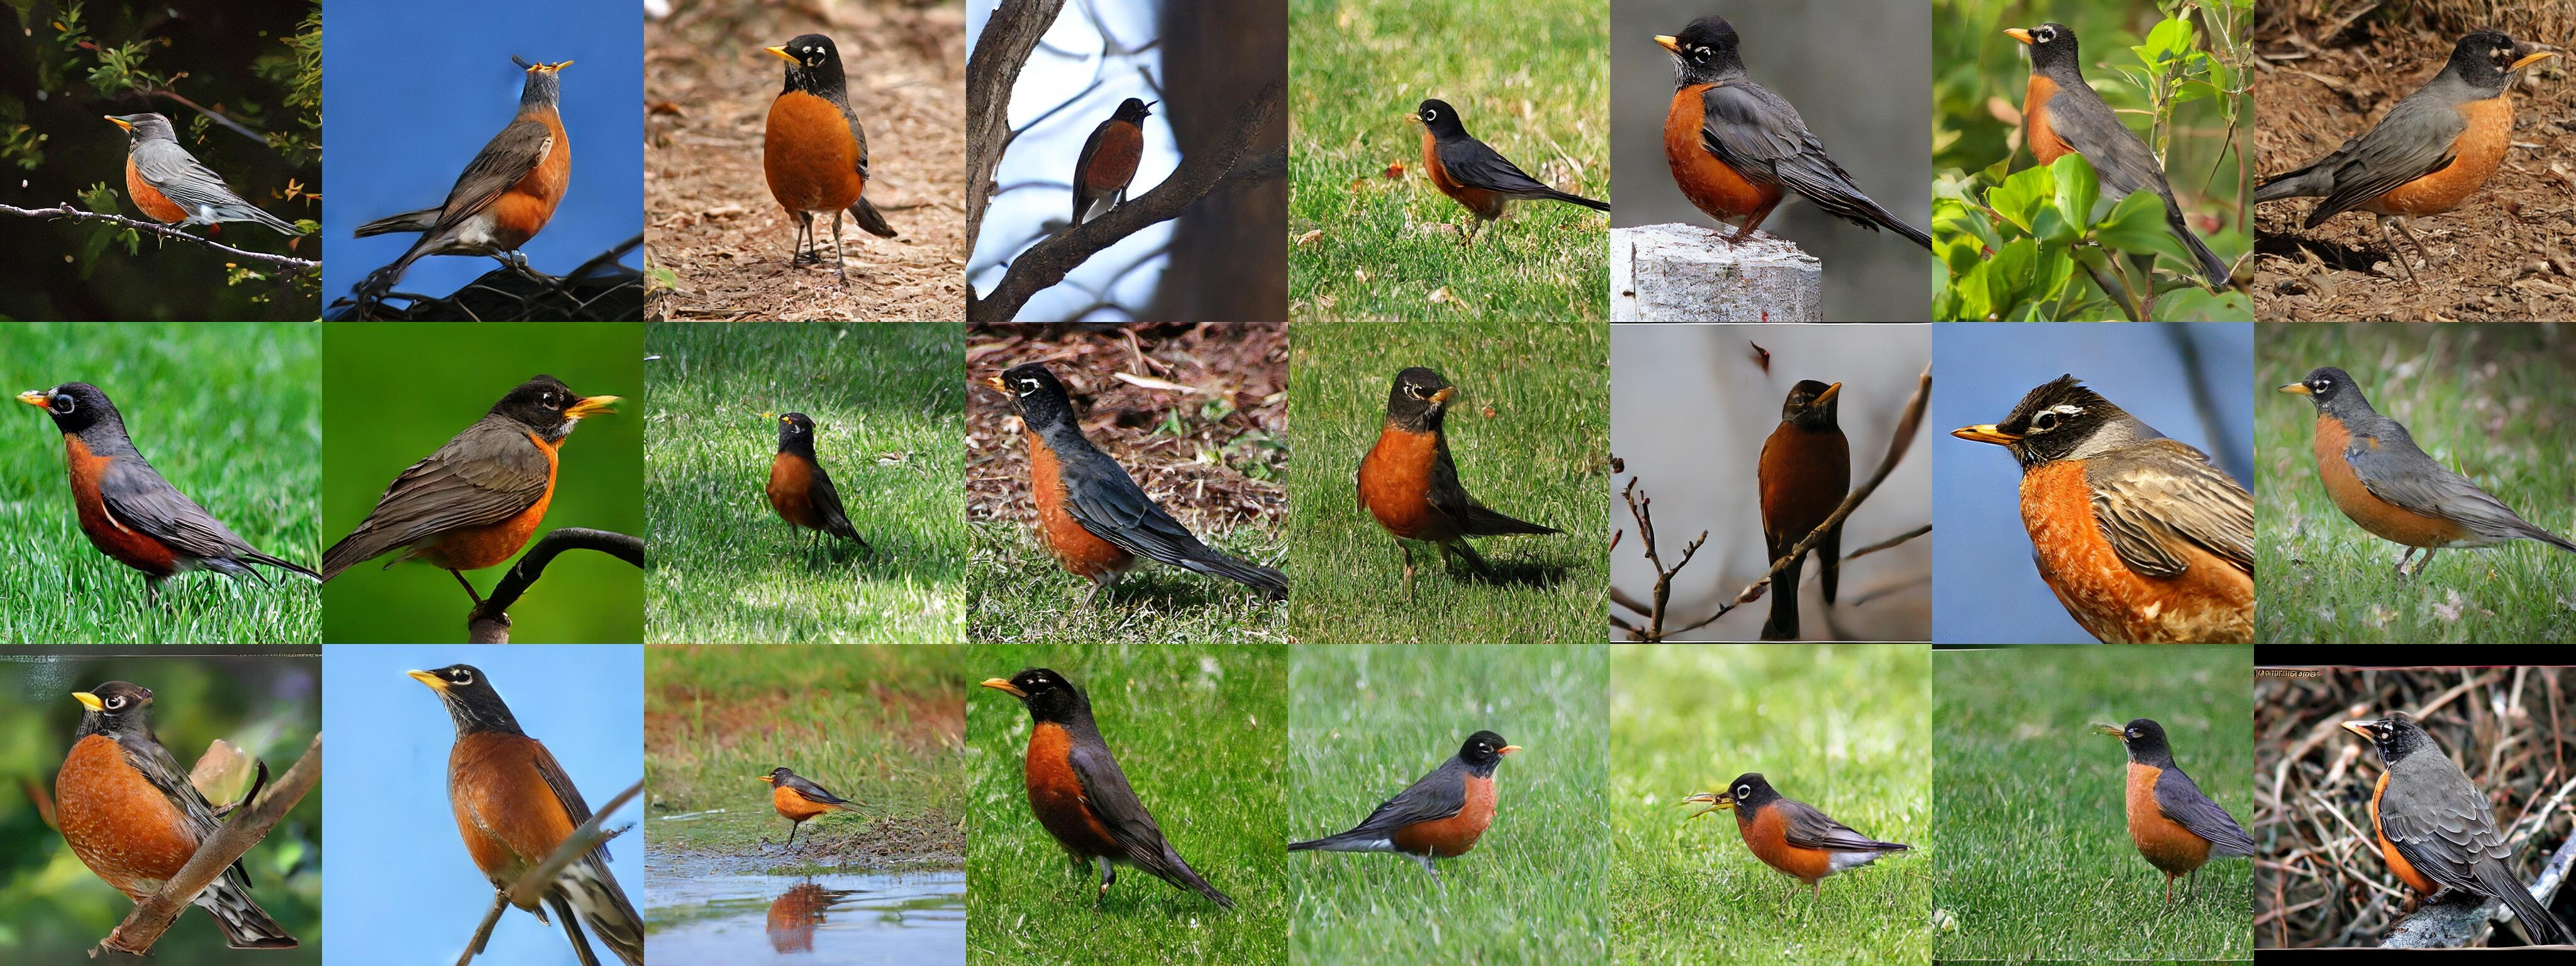
\includegraphics[width=\linewidth]{figures/samples-appendix-1step/15_batch.jpg} \\
	\end{minipage} \\
 
        \vspace{.2cm}
        
 	\begin{minipage}{0.05\linewidth}
         \rotatebox{90}{\small{Class 29 (axolotl), guidance 1.9}}
		\centering
	\end{minipage}
	\begin{minipage}{0.93\linewidth}
		\centering
        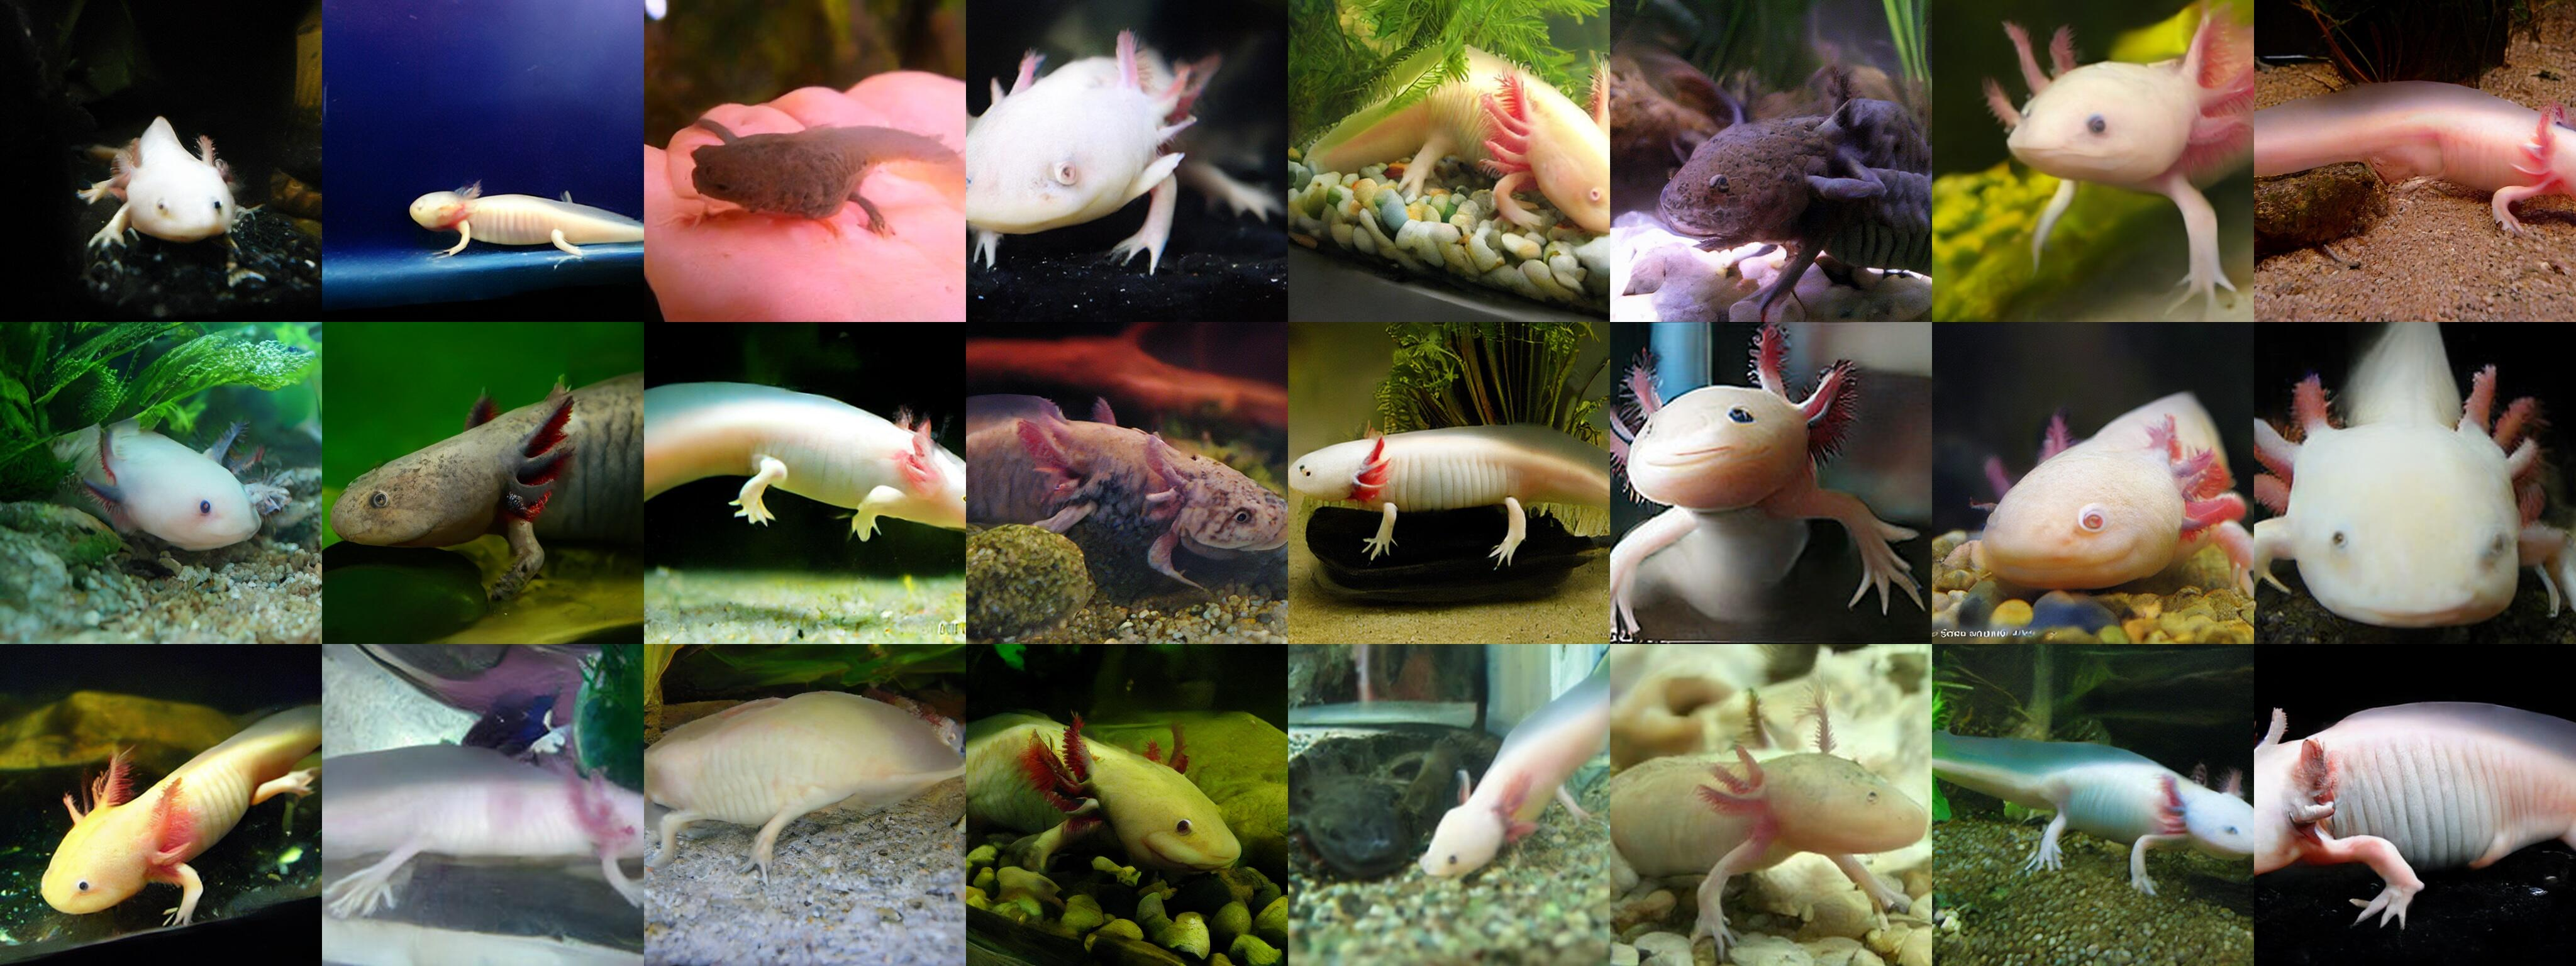
\includegraphics[width=\linewidth]{figures/samples-appendix-1step/29_batch.jpg}\\
	\end{minipage} \\
 
        \vspace{.2cm}
        
 	\begin{minipage}{0.05\linewidth}
         \rotatebox{90}{\small{Class 33 (loggerhead), guidance 1.9}}
		\centering
	\end{minipage}
	\begin{minipage}{0.93\linewidth}
		\centering
        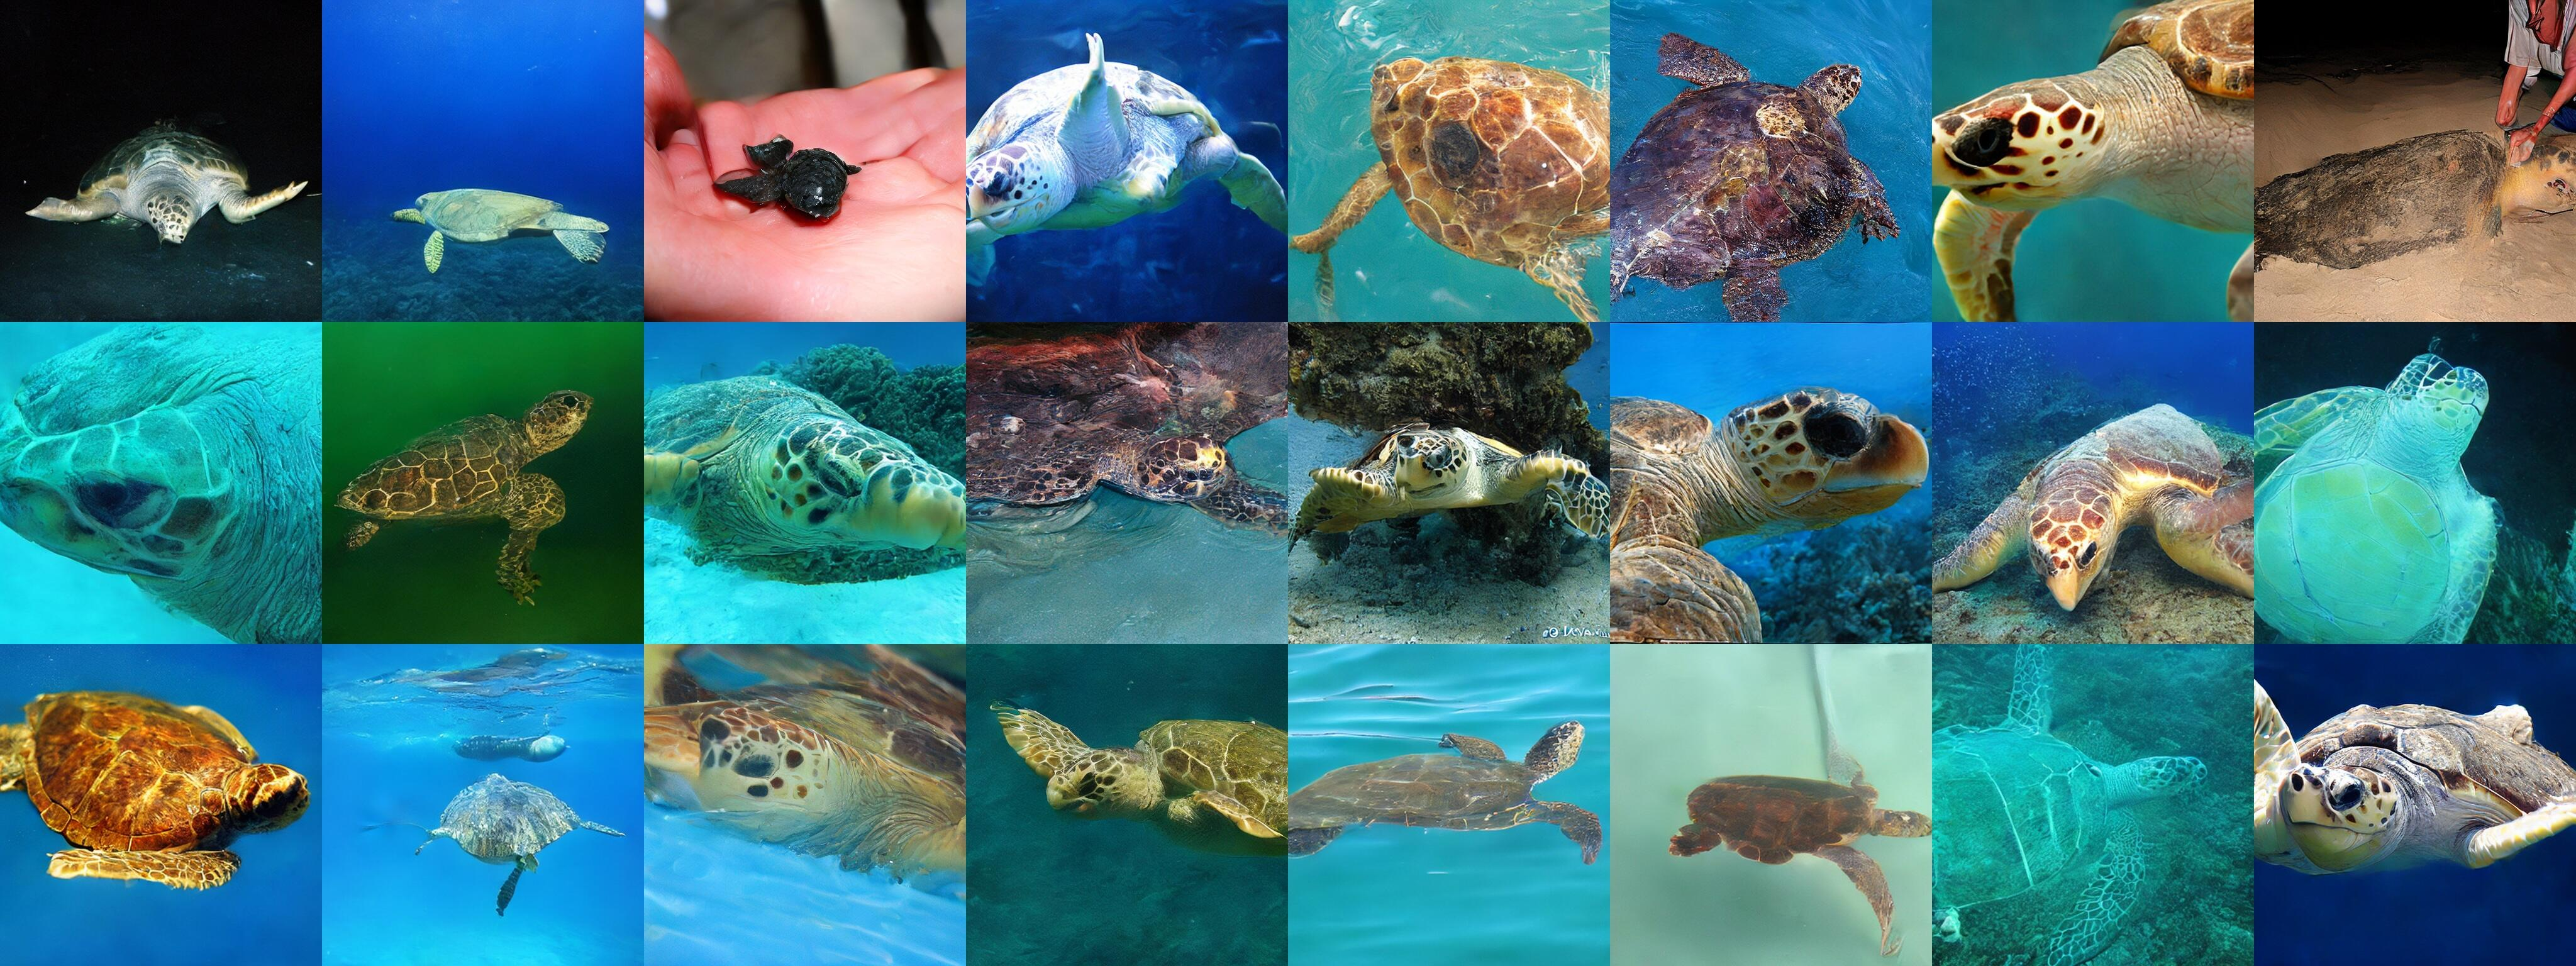
\includegraphics[width=\linewidth]{figures/samples-appendix-1step/33_batch.jpg}\\
	\end{minipage} \\
        \vspace{.2cm}
        
 	\begin{minipage}{0.05\linewidth}
         \rotatebox{90}{\small{Class 88 (macaw), guidance 1.9}}
		\centering
	\end{minipage}
	\begin{minipage}{0.93\linewidth}
		\centering
        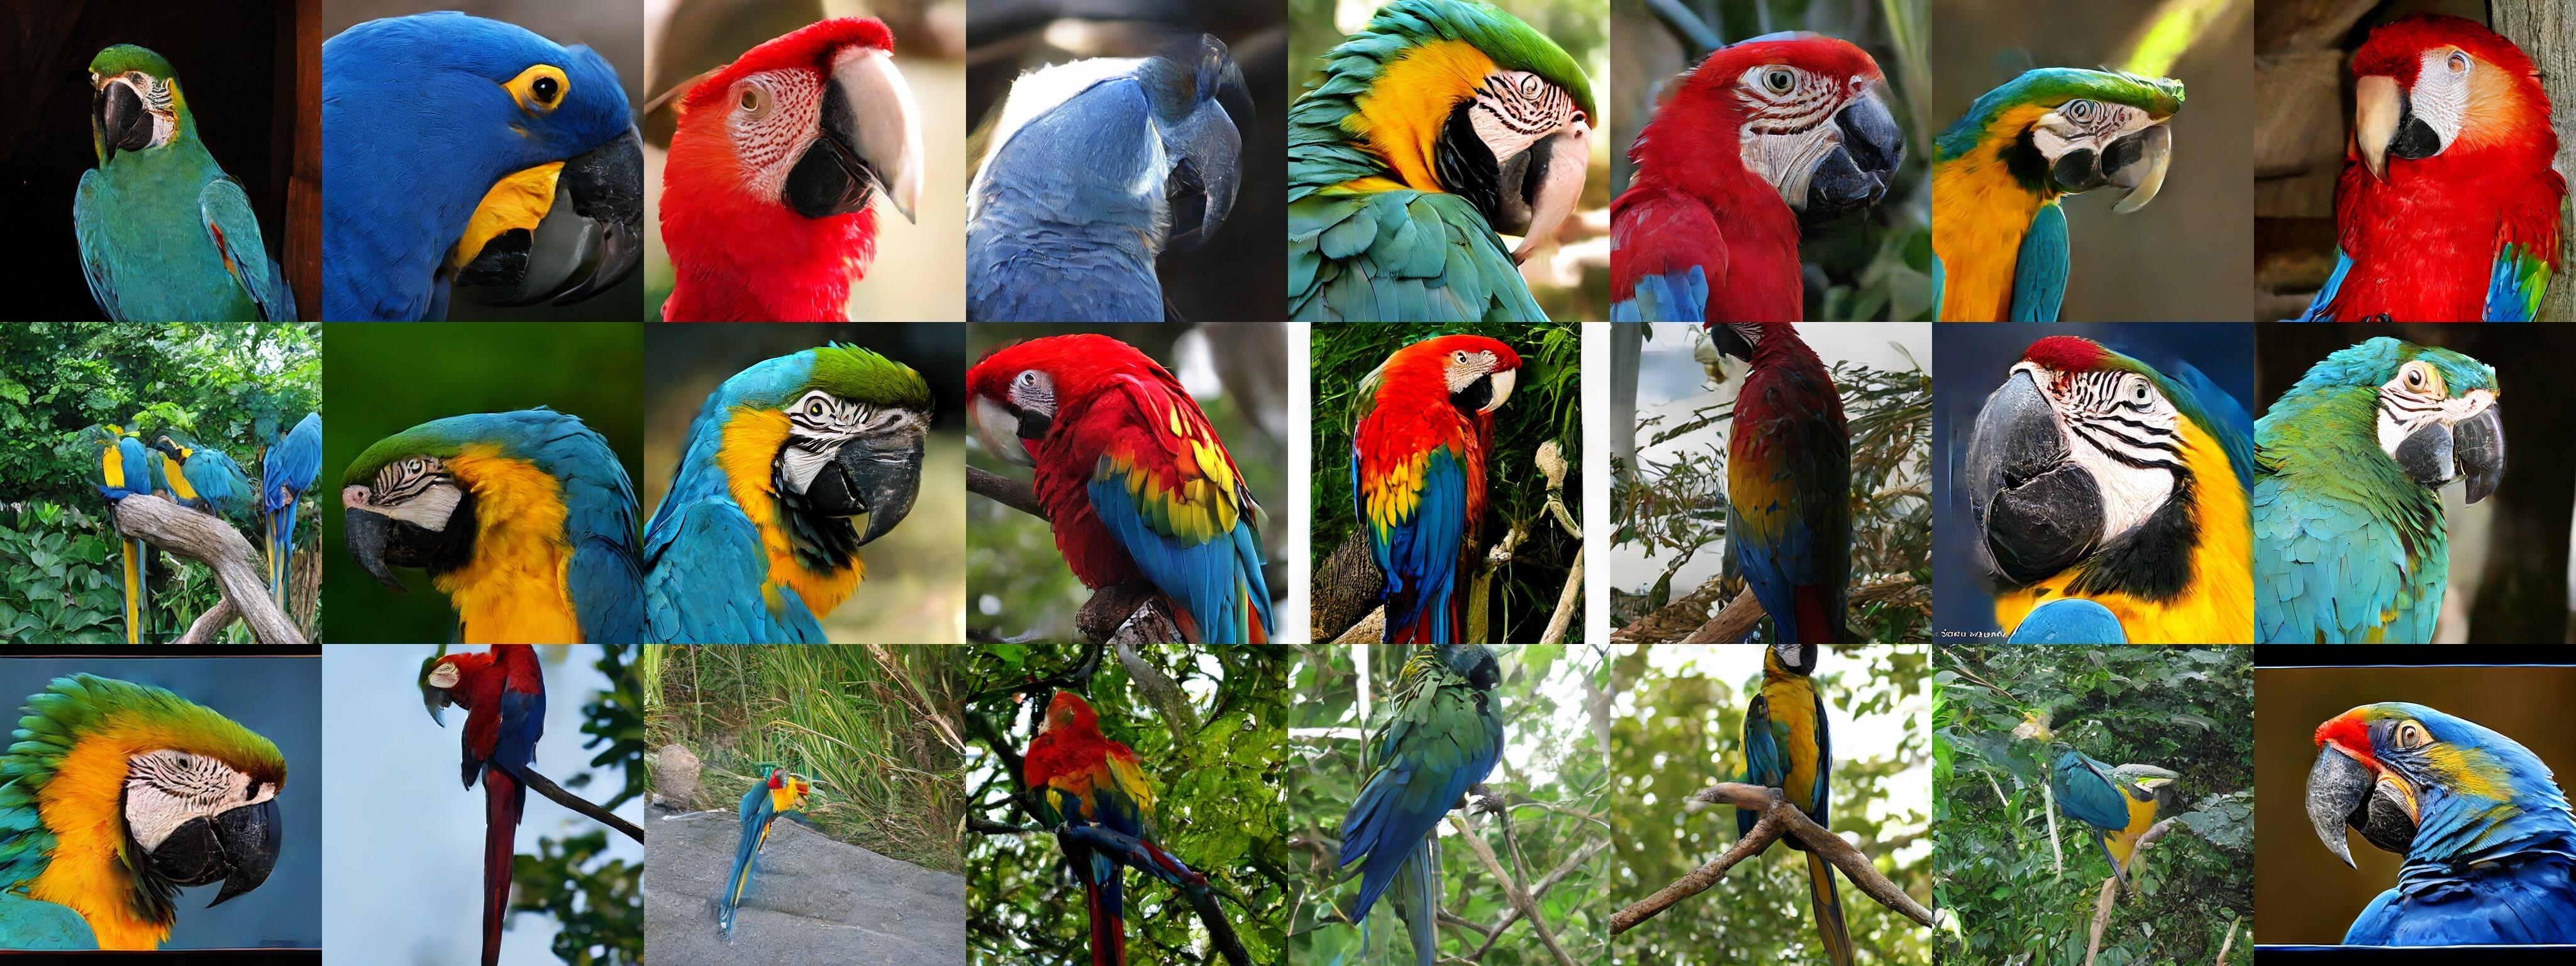
\includegraphics[width=\linewidth]{figures/samples-appendix-1step/88_batch.jpg}\\
	\end{minipage} \\

	\caption{\small{Uncurated 1-step samples generated by our sCD-XXL trained on ImageNet 512$\times$512.}
	\label{fig:appendix:samples-1-1step}}
\end{figure}


\begin{figure}[H]
	\begin{minipage}{0.05\linewidth}
         \rotatebox{90}{\small{Class 15 (robin), guidance 1.9}}
		\centering
	\end{minipage}
	\begin{minipage}{0.93\linewidth}
		\centering
        
\includegraphics[width=\linewidth]{figures/samples-appendix/15_batch.jpg} \\
	\end{minipage} \\
 
        \vspace{.2cm}
        
 	\begin{minipage}{0.05\linewidth}
         \rotatebox{90}{\small{Class 29 (axolotl), guidance 1.9}}
		\centering
	\end{minipage}
	\begin{minipage}{0.93\linewidth}
		\centering
        
\includegraphics[width=\linewidth]{figures/samples-appendix/29_batch.jpg}\\
	\end{minipage} \\
 
        \vspace{.2cm}
        
 	\begin{minipage}{0.05\linewidth}
         \rotatebox{90}{\small{Class 33 (loggerhead), guidance 1.9}}
		\centering
	\end{minipage}
	\begin{minipage}{0.93\linewidth}
		\centering
        
\includegraphics[width=\linewidth]{figures/samples-appendix/33_batch.jpg}\\
	\end{minipage} \\
        \vspace{.2cm}
        
 	\begin{minipage}{0.05\linewidth}
         \rotatebox{90}{\small{Class 88 (macaw), guidance 1.9}}
		\centering
	\end{minipage}
	\begin{minipage}{0.93\linewidth}
		\centering
        
\includegraphics[width=\linewidth]{figures/samples-appendix/88_batch.jpg}\\
	\end{minipage} \\

	\caption{\small{Uncurated 2-step samples generated by our sCD-XXL trained on ImageNet 512$\times$512.}
	\label{fig:appendix:samples-1}}
\end{figure}


\begin{figure}[H]
 	\begin{minipage}{0.05\linewidth}
         \rotatebox{90}{\small{Class 127 (white stork), guidance 1.9}}
		\centering
	\end{minipage}
	\begin{minipage}{0.93\linewidth}
		\centering
        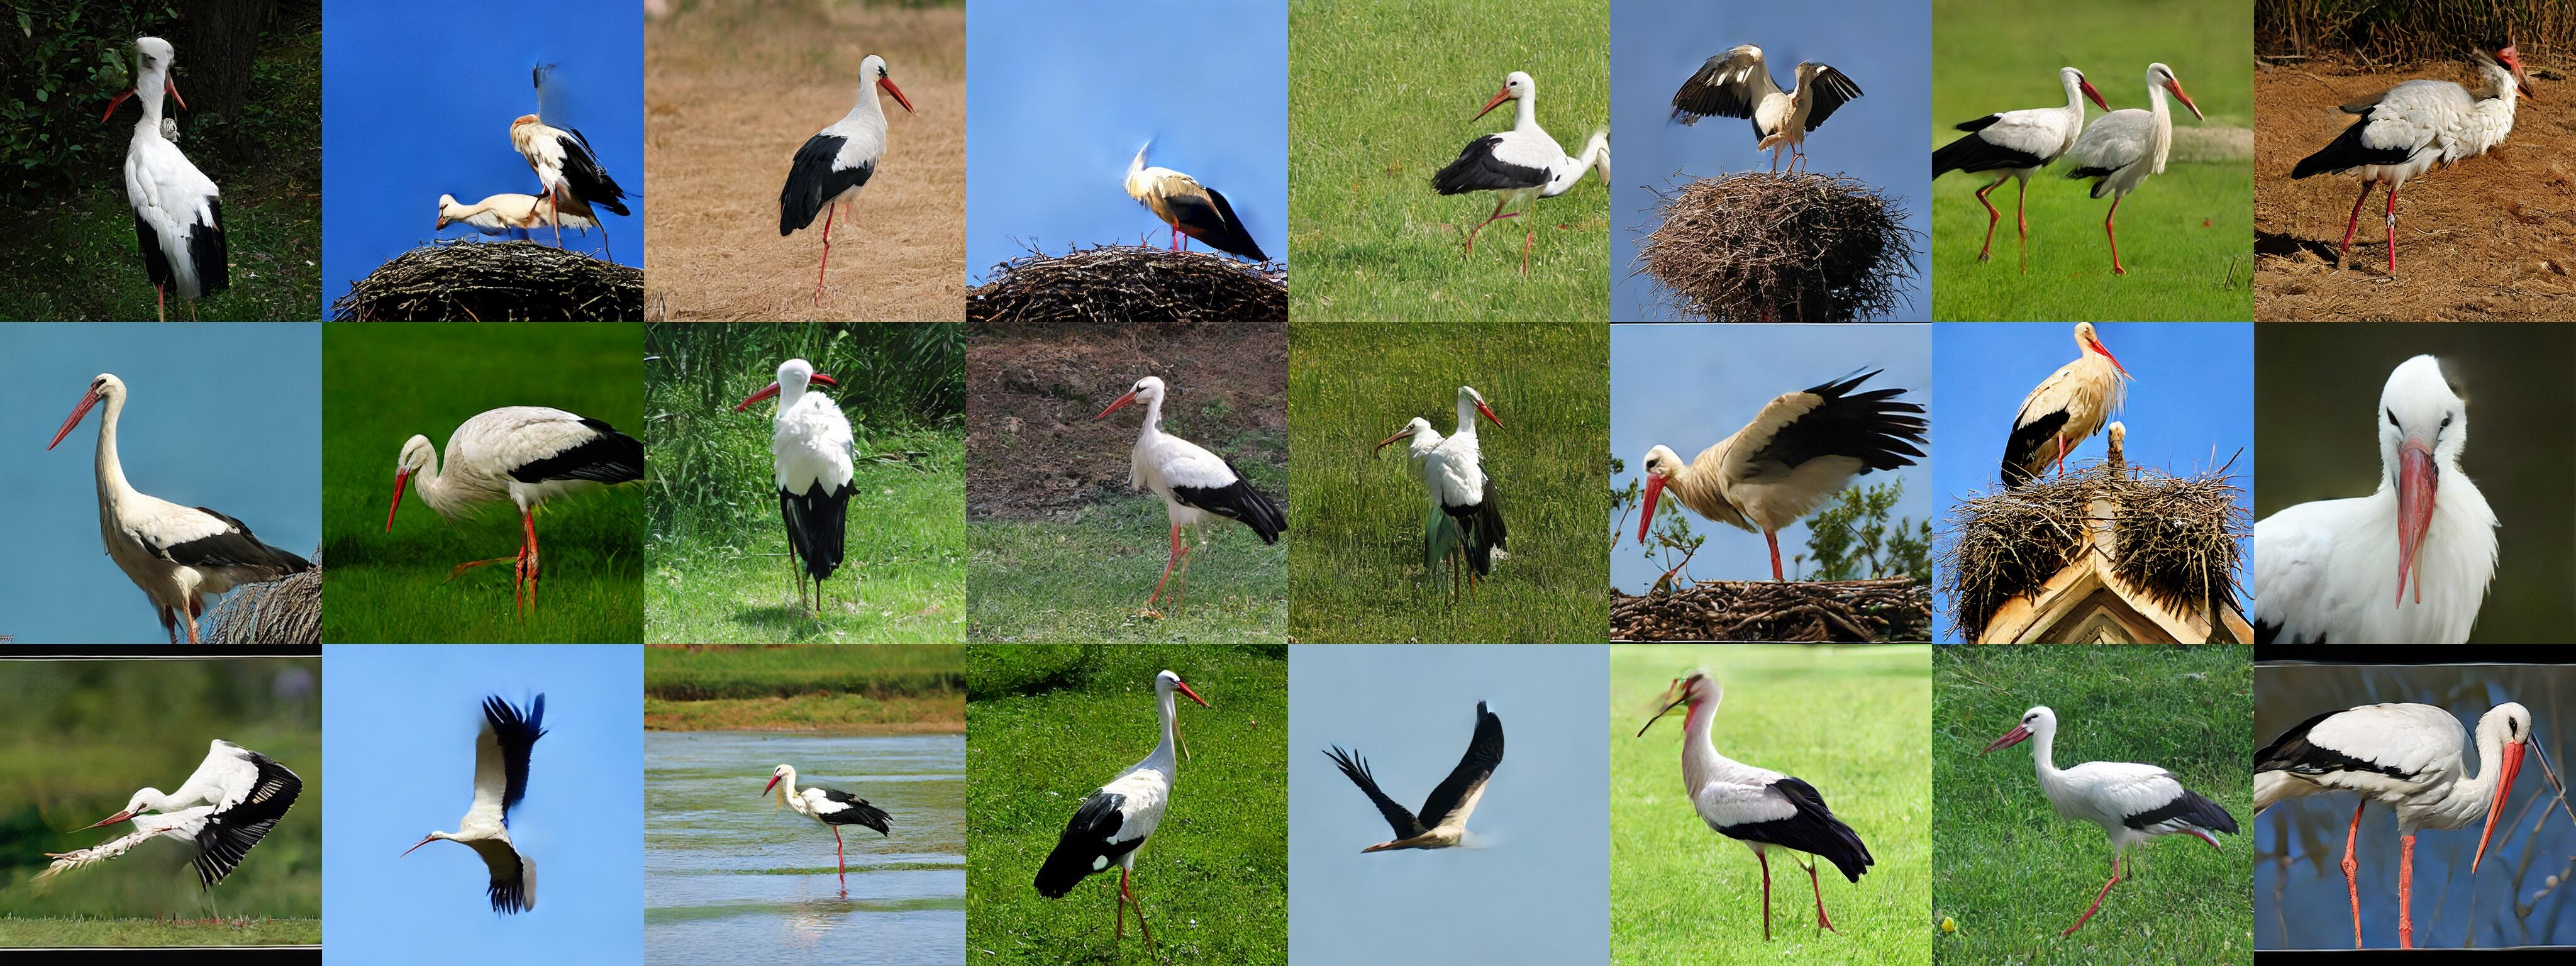
\includegraphics[width=\linewidth]{figures/samples-appendix-1step/127_batch.jpg}\\
	\end{minipage} \\

        \vspace{.2cm}
 	\begin{minipage}{0.05\linewidth}
         \rotatebox{90}{\small{Class 323 (monarch), guidance 1.9}}
		\centering
	\end{minipage}
	\begin{minipage}{0.93\linewidth}
		\centering
        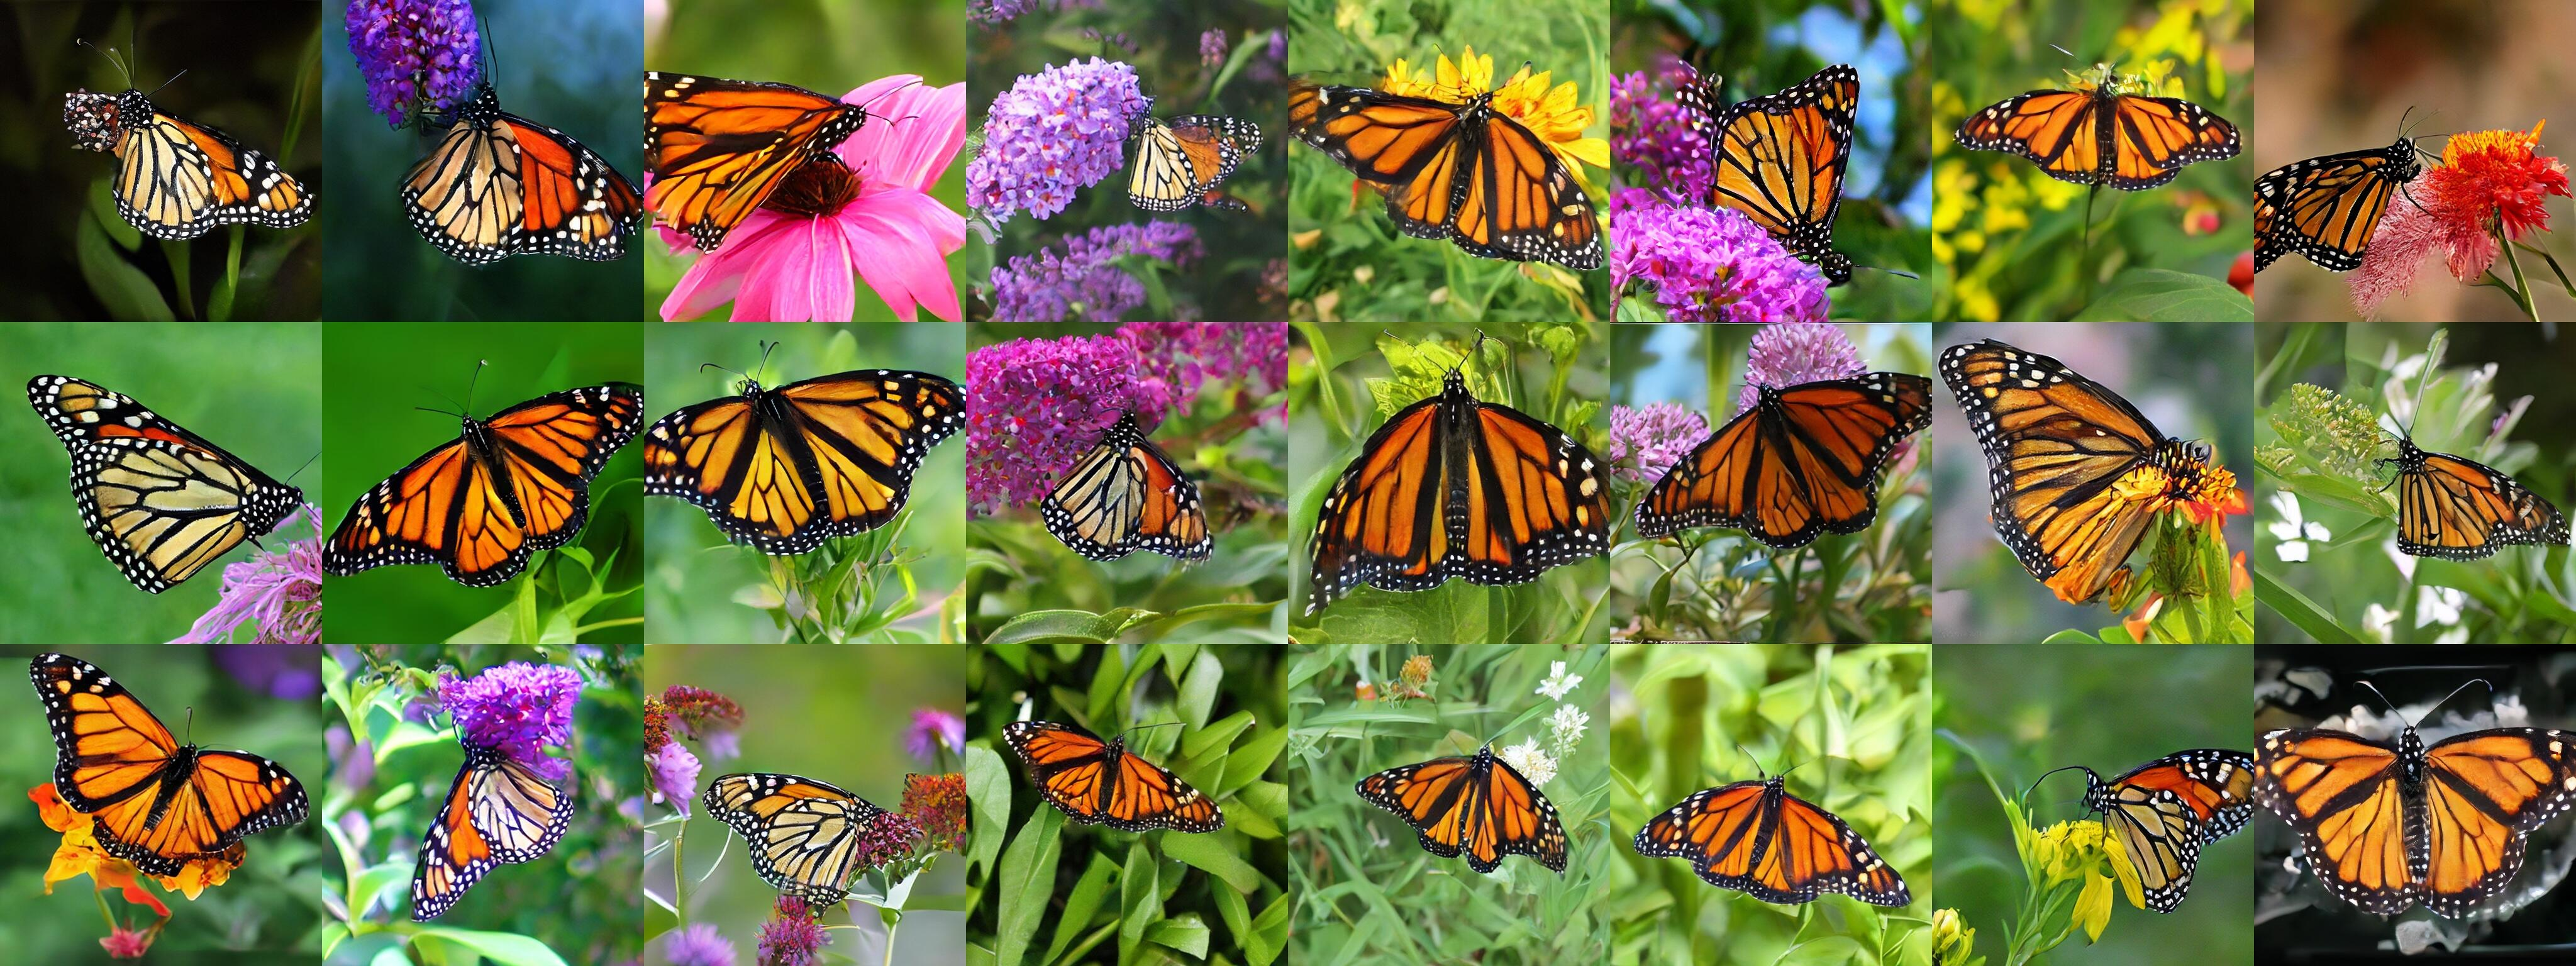
\includegraphics[width=\linewidth]{figures/samples-appendix-1step/323_batch.jpg}\\
	\end{minipage} \\

                \vspace{.2cm}
 	\begin{minipage}{0.05\linewidth}
         \rotatebox{90}{\small{Class 387 (lesser panda), guidance 1.9}}
		\centering
	\end{minipage}
	\begin{minipage}{0.93\linewidth}
		\centering
        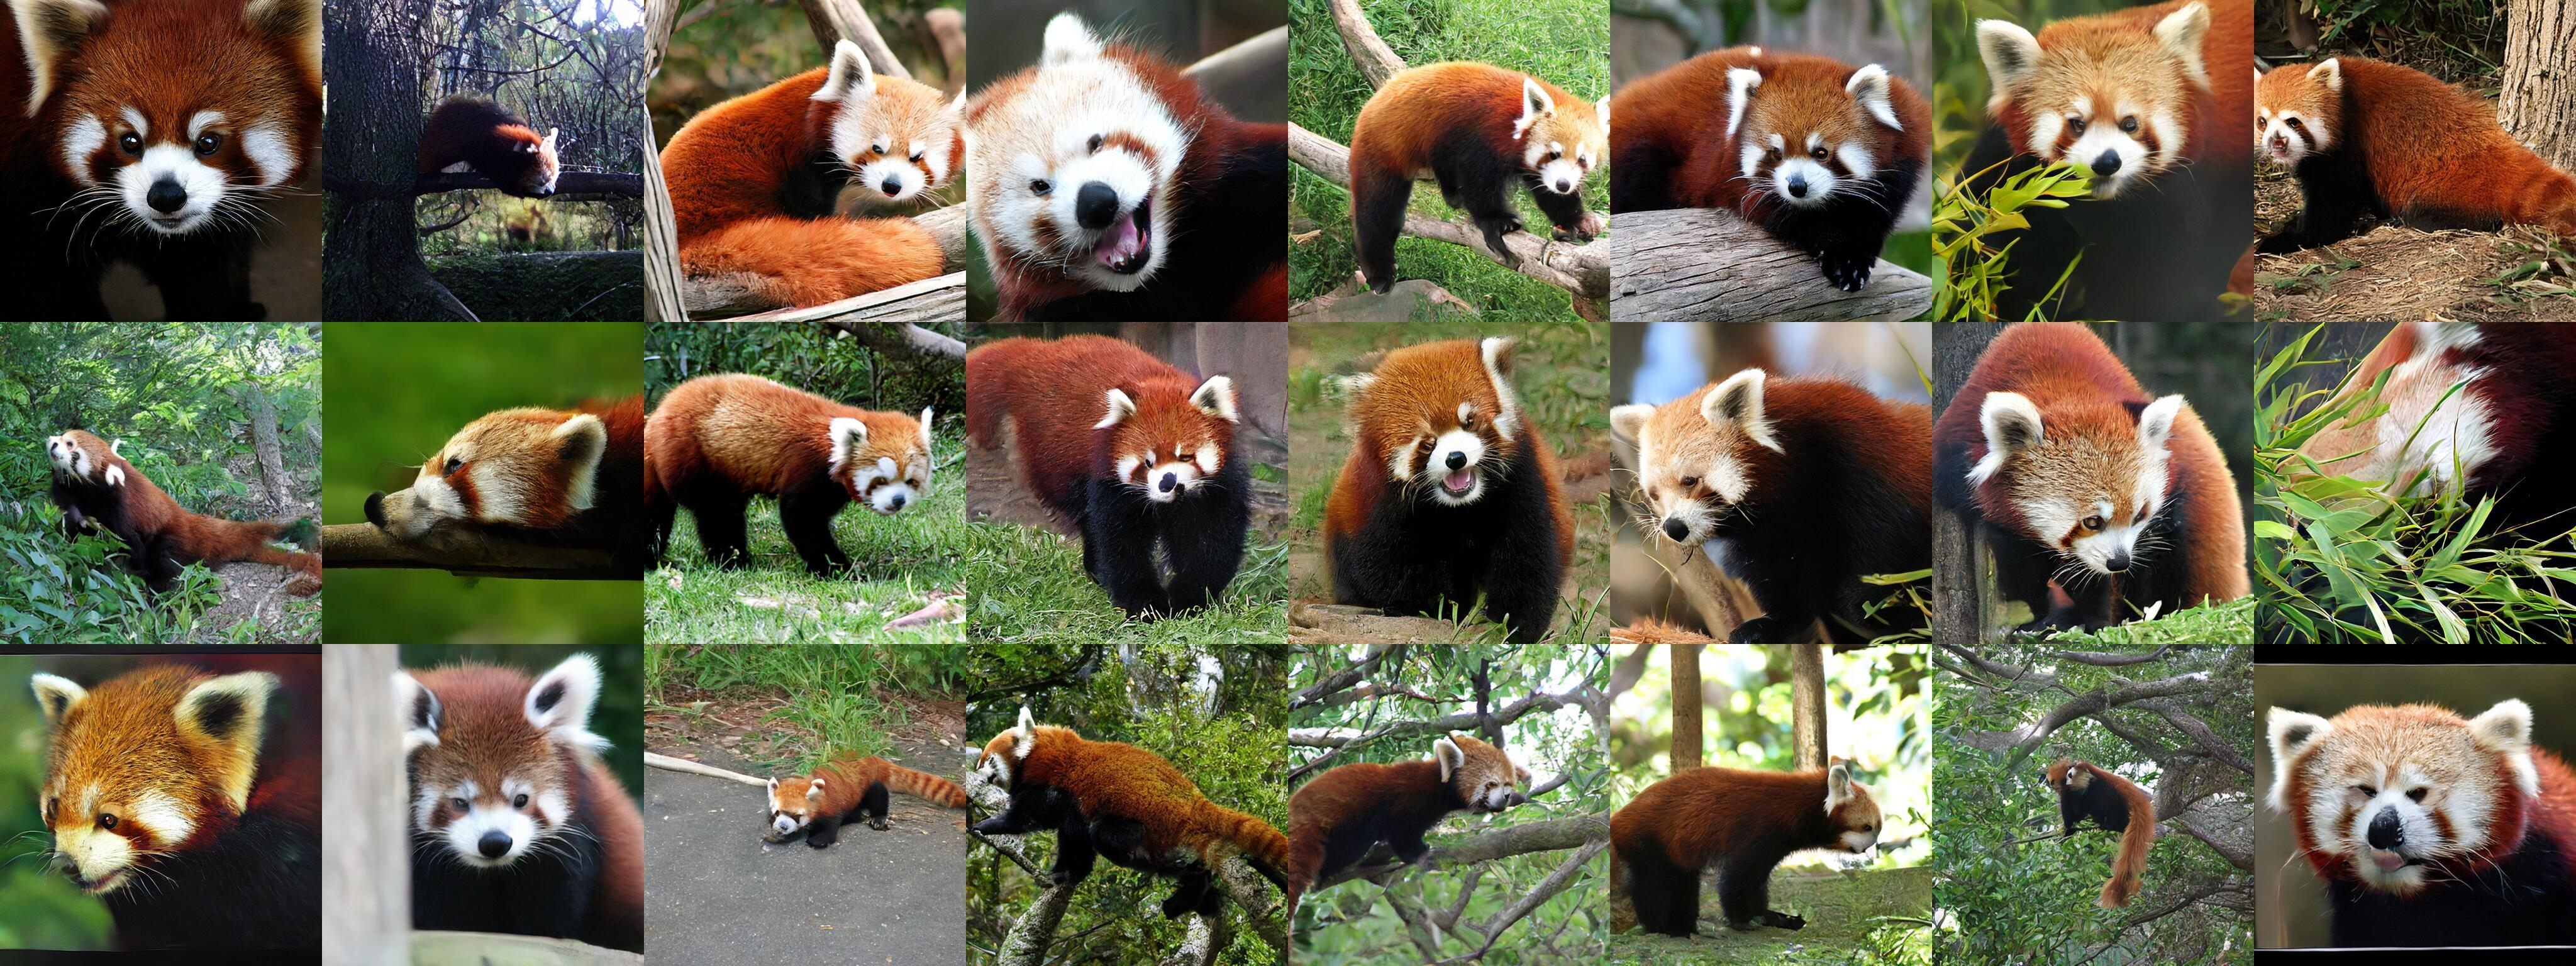
\includegraphics[width=\linewidth]{figures/samples-appendix-1step/387_batch.jpg}\\
	\end{minipage} \\
                \vspace{.2cm}
 	\begin{minipage}{0.05\linewidth}
         \rotatebox{90}{\small{Class 388 (giant panda), guidance 1.9}}
		\centering
	\end{minipage}
	\begin{minipage}{0.93\linewidth}
		\centering
        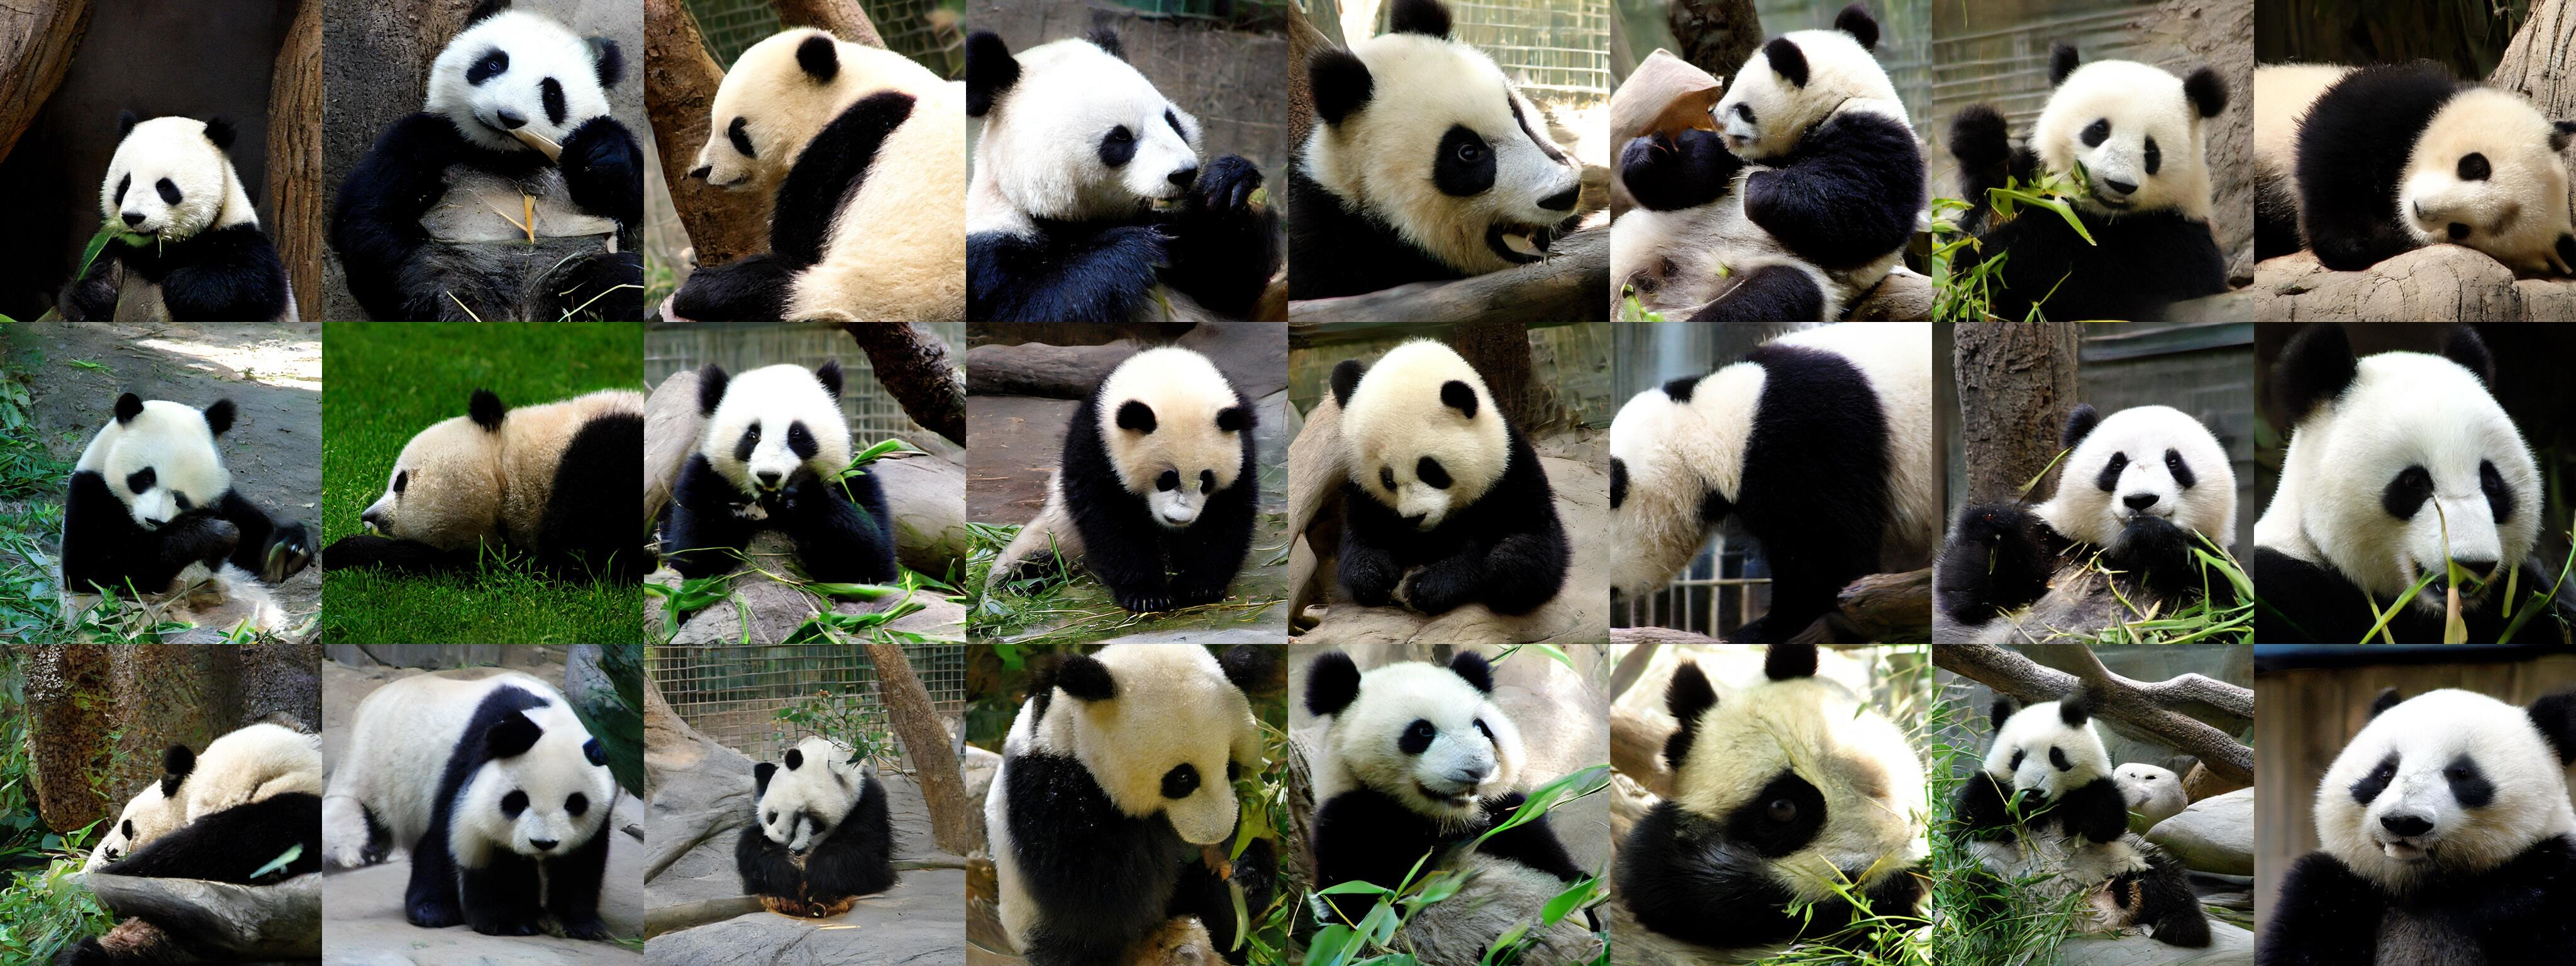
\includegraphics[width=\linewidth]{figures/samples-appendix-1step/388_batch.jpg}\\
	\end{minipage} \\

	\caption{\small{Uncurated 1-step samples generated by our sCD-XXL trained on ImageNet 512$\times$512.}
	\label{fig:appendix:samples-2-1step}}
\end{figure}


\begin{figure}[H]
 	\begin{minipage}{0.05\linewidth}
         \rotatebox{90}{\small{Class 127 (white stork), guidance 1.9}}
		\centering
	\end{minipage}
	\begin{minipage}{0.93\linewidth}
		\centering
        
\includegraphics[width=\linewidth]{figures/samples-appendix/127_batch.jpg}\\
	\end{minipage} \\

        \vspace{.2cm}
 	\begin{minipage}{0.05\linewidth}
         \rotatebox{90}{\small{Class 323 (monarch), guidance 1.9}}
		\centering
	\end{minipage}
	\begin{minipage}{0.93\linewidth}
		\centering
        
\includegraphics[width=\linewidth]{figures/samples-appendix/323_batch.jpg}\\
	\end{minipage} \\

                \vspace{.2cm}
 	\begin{minipage}{0.05\linewidth}
         \rotatebox{90}{\small{Class 387 (lesser panda), guidance 1.9}}
		\centering
	\end{minipage}
	\begin{minipage}{0.93\linewidth}
		\centering
        
\includegraphics[width=\linewidth]{figures/samples-appendix/387_batch.jpg}\\
	\end{minipage} \\
                \vspace{.2cm}
 	\begin{minipage}{0.05\linewidth}
         \rotatebox{90}{\small{Class 388 (giant panda), guidance 1.9}}
		\centering
	\end{minipage}
	\begin{minipage}{0.93\linewidth}
		\centering
        
\includegraphics[width=\linewidth]{figures/samples-appendix/388_batch.jpg}\\
	\end{minipage} \\

	\caption{\small{Uncurated 2-step samples generated by our sCD-XXL trained on ImageNet 512$\times$512.}
	\label{fig:appendix:samples-2}}
\end{figure}


\begin{figure}[H]
 	\begin{minipage}{0.05\linewidth}
         \rotatebox{90}{\small{Class 417 (balloon), guidance 1.9}}
		\centering
	\end{minipage}
	\begin{minipage}{0.93\linewidth}
		\centering
        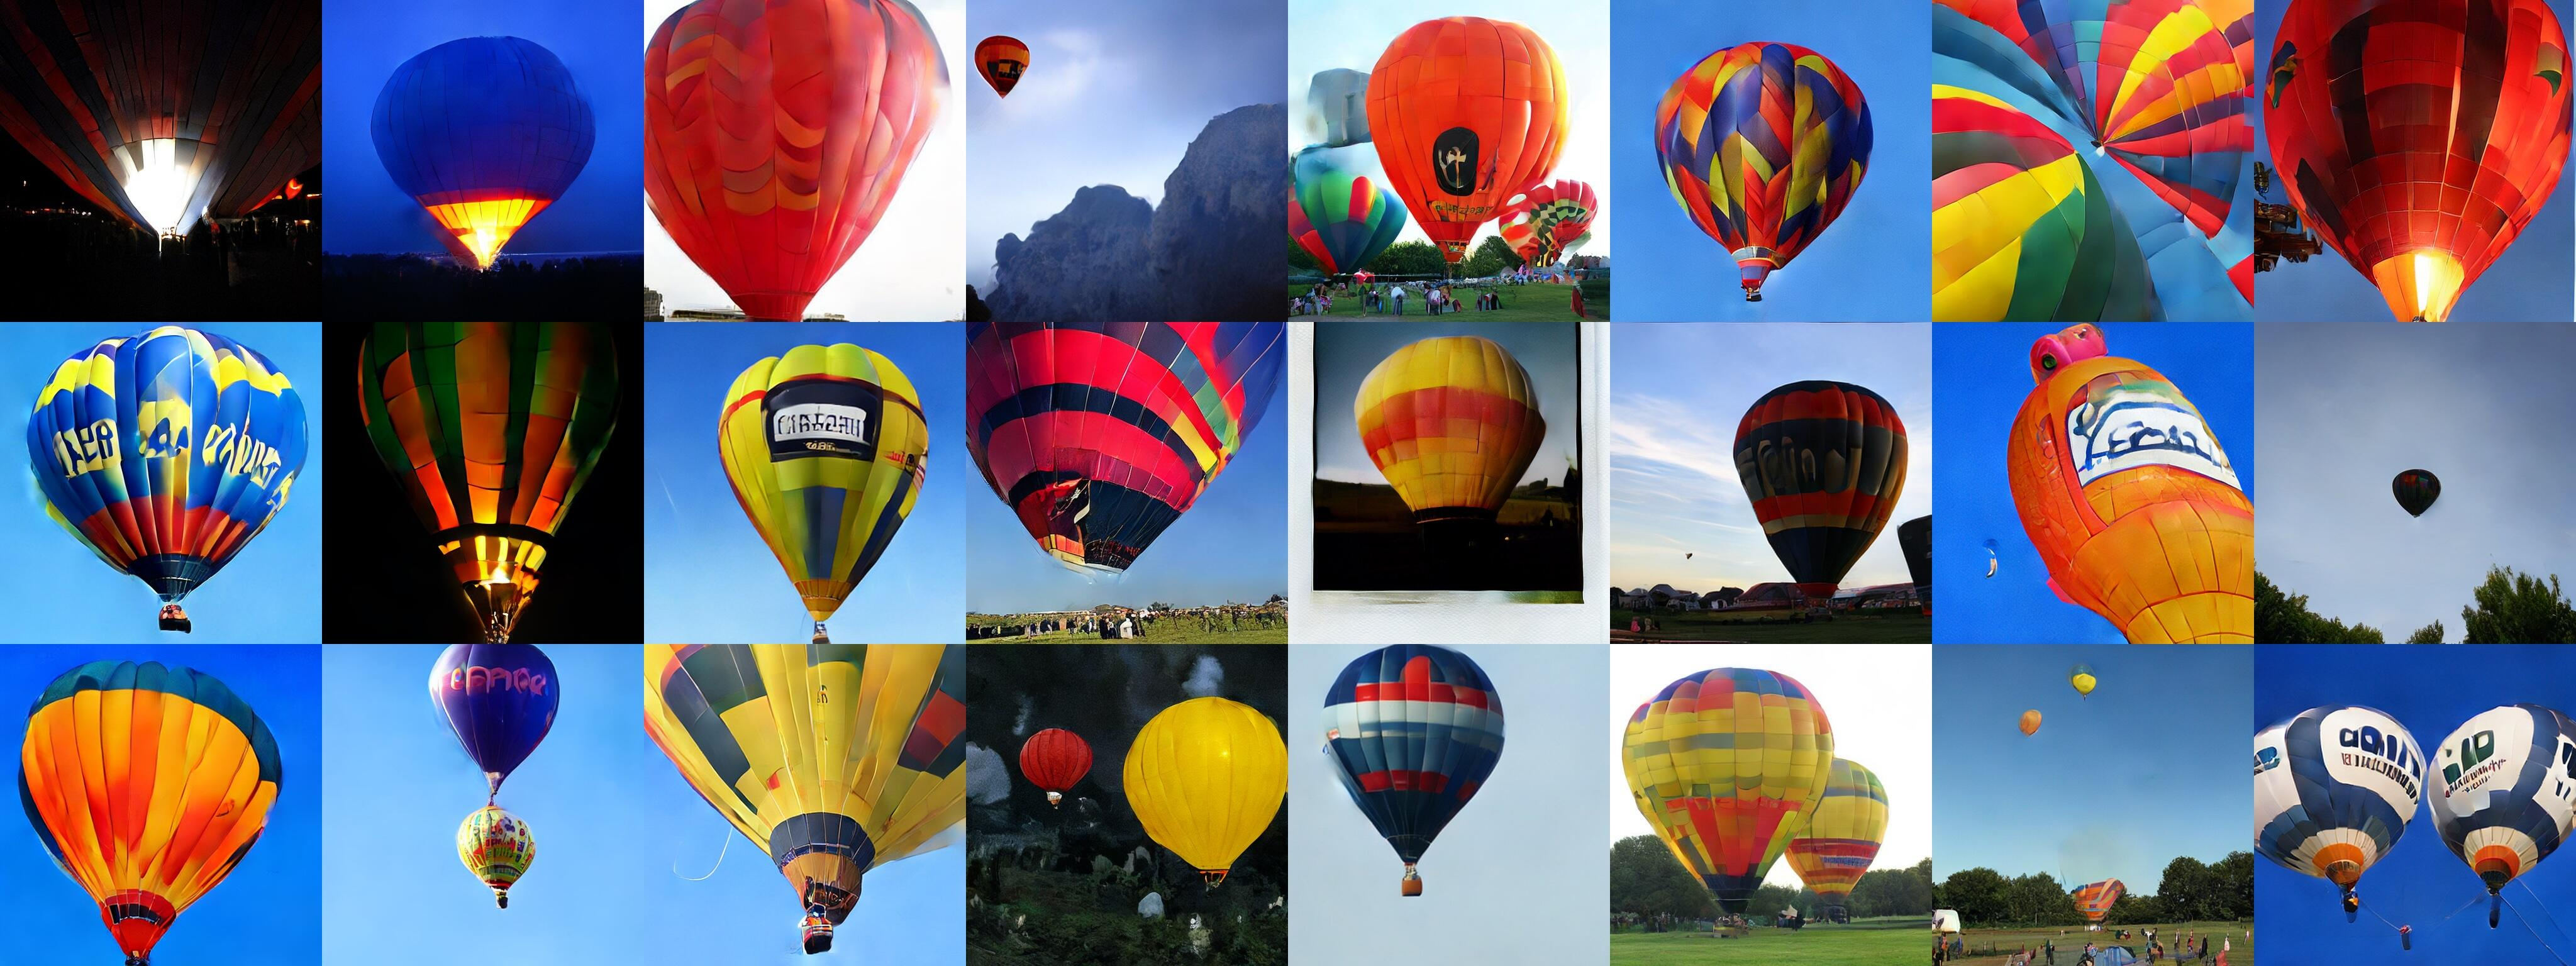
\includegraphics[width=\linewidth]{figures/samples-appendix-1step/417_batch.jpg}\\
	\end{minipage} \\

        \vspace{.2cm}
 	\begin{minipage}{0.05\linewidth}
         \rotatebox{90}{\small{Class 425 (barn), guidance 1.9}}
		\centering
	\end{minipage}
	\begin{minipage}{0.93\linewidth}
		\centering
        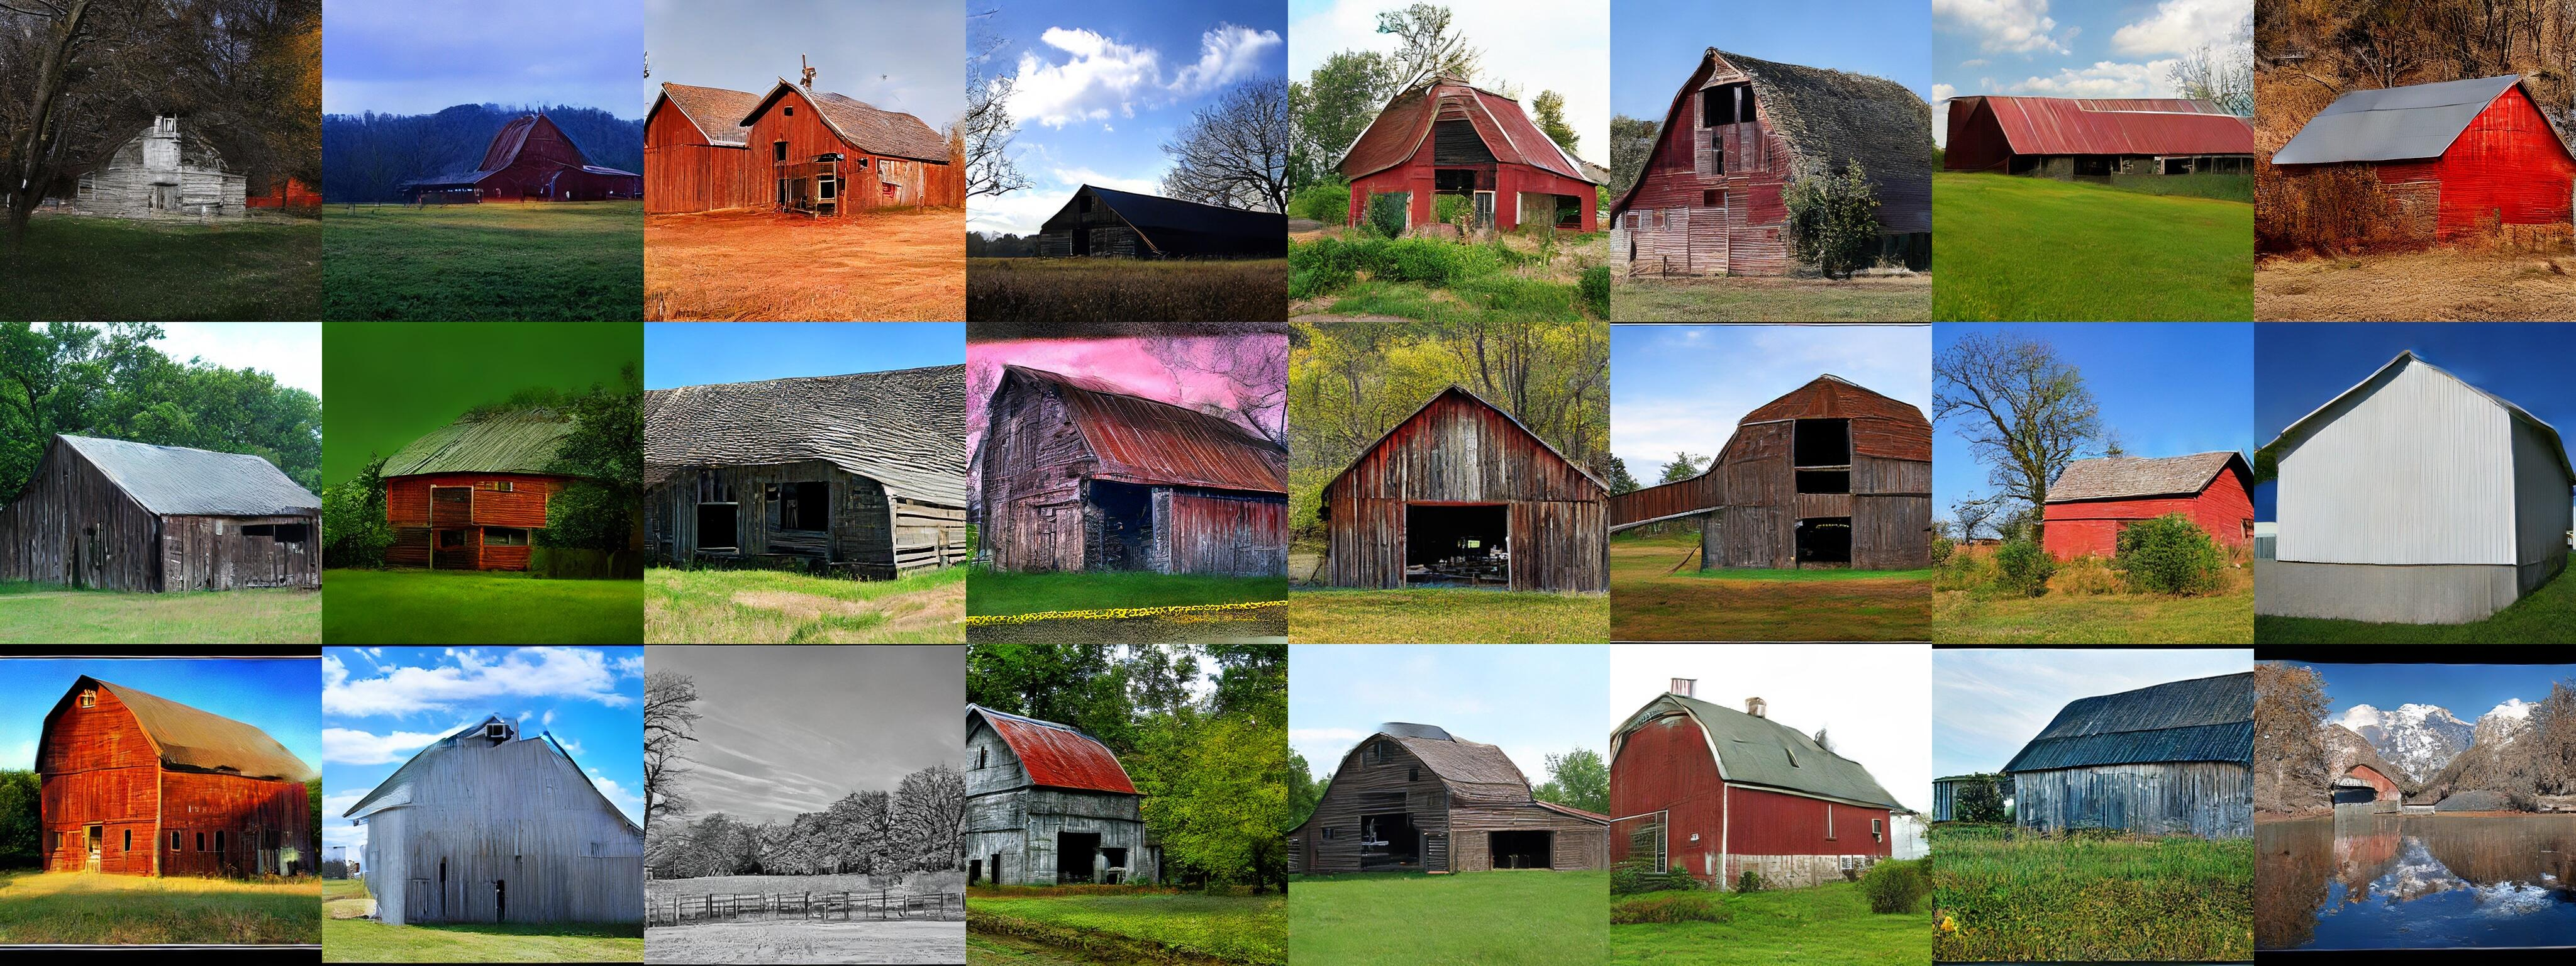
\includegraphics[width=\linewidth]{figures/samples-appendix-1step/425_batch.jpg}\\
	\end{minipage} \\

                \vspace{.2cm}
 	\begin{minipage}{0.05\linewidth}
         \rotatebox{90}{\small{Class 933 (cheeseburger), guidance 1.9}}
		\centering
	\end{minipage}
	\begin{minipage}{0.93\linewidth}
		\centering
        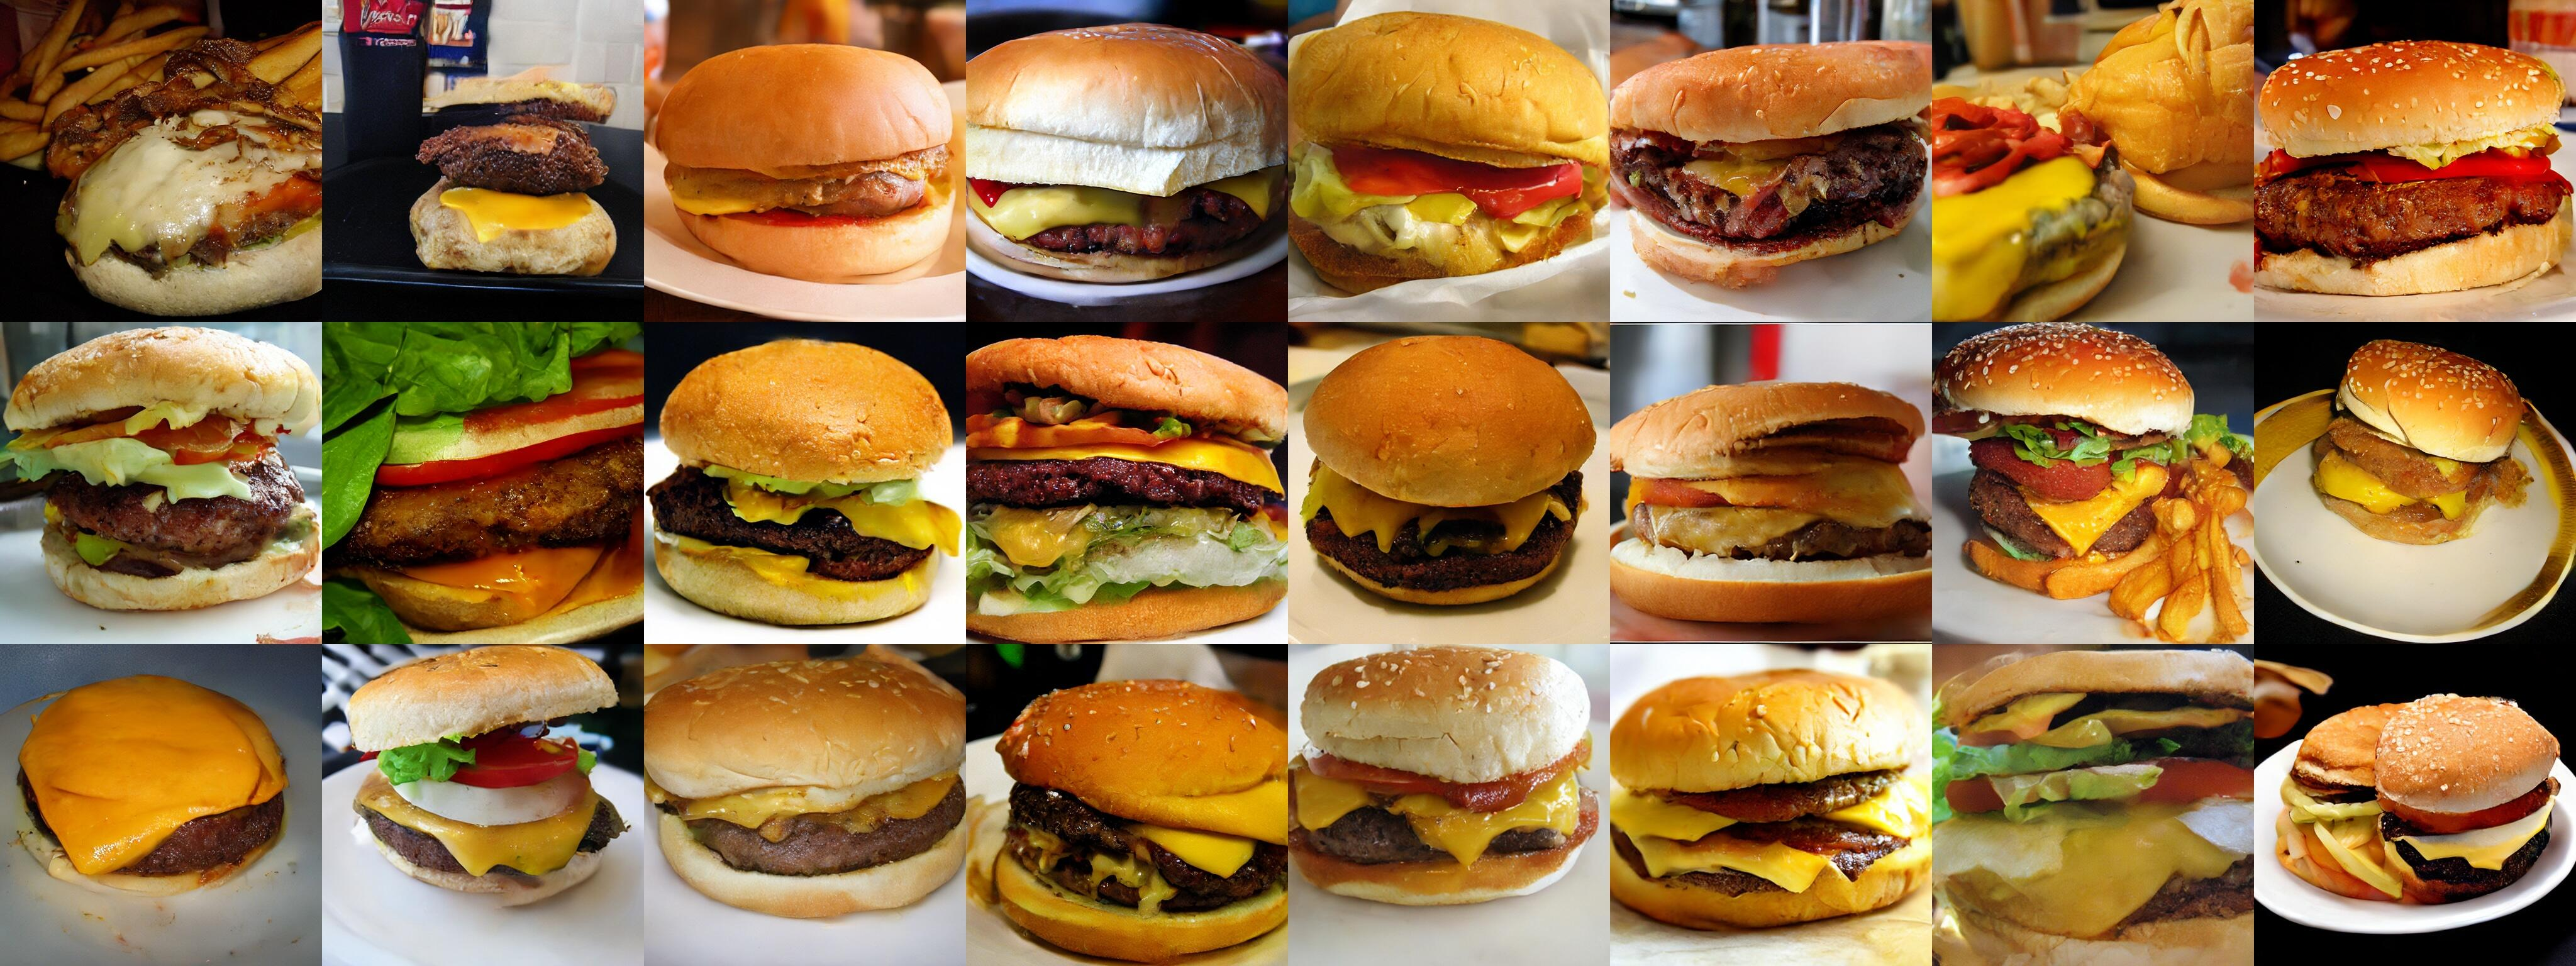
\includegraphics[width=\linewidth]{figures/samples-appendix-1step/933_batch.jpg}\\
	\end{minipage} \\
                \vspace{.2cm}
 	\begin{minipage}{0.05\linewidth}
         \rotatebox{90}{\small{Class 973 (coral reef), guidance 1.9}}
		\centering
	\end{minipage}
	\begin{minipage}{0.93\linewidth}
		\centering
        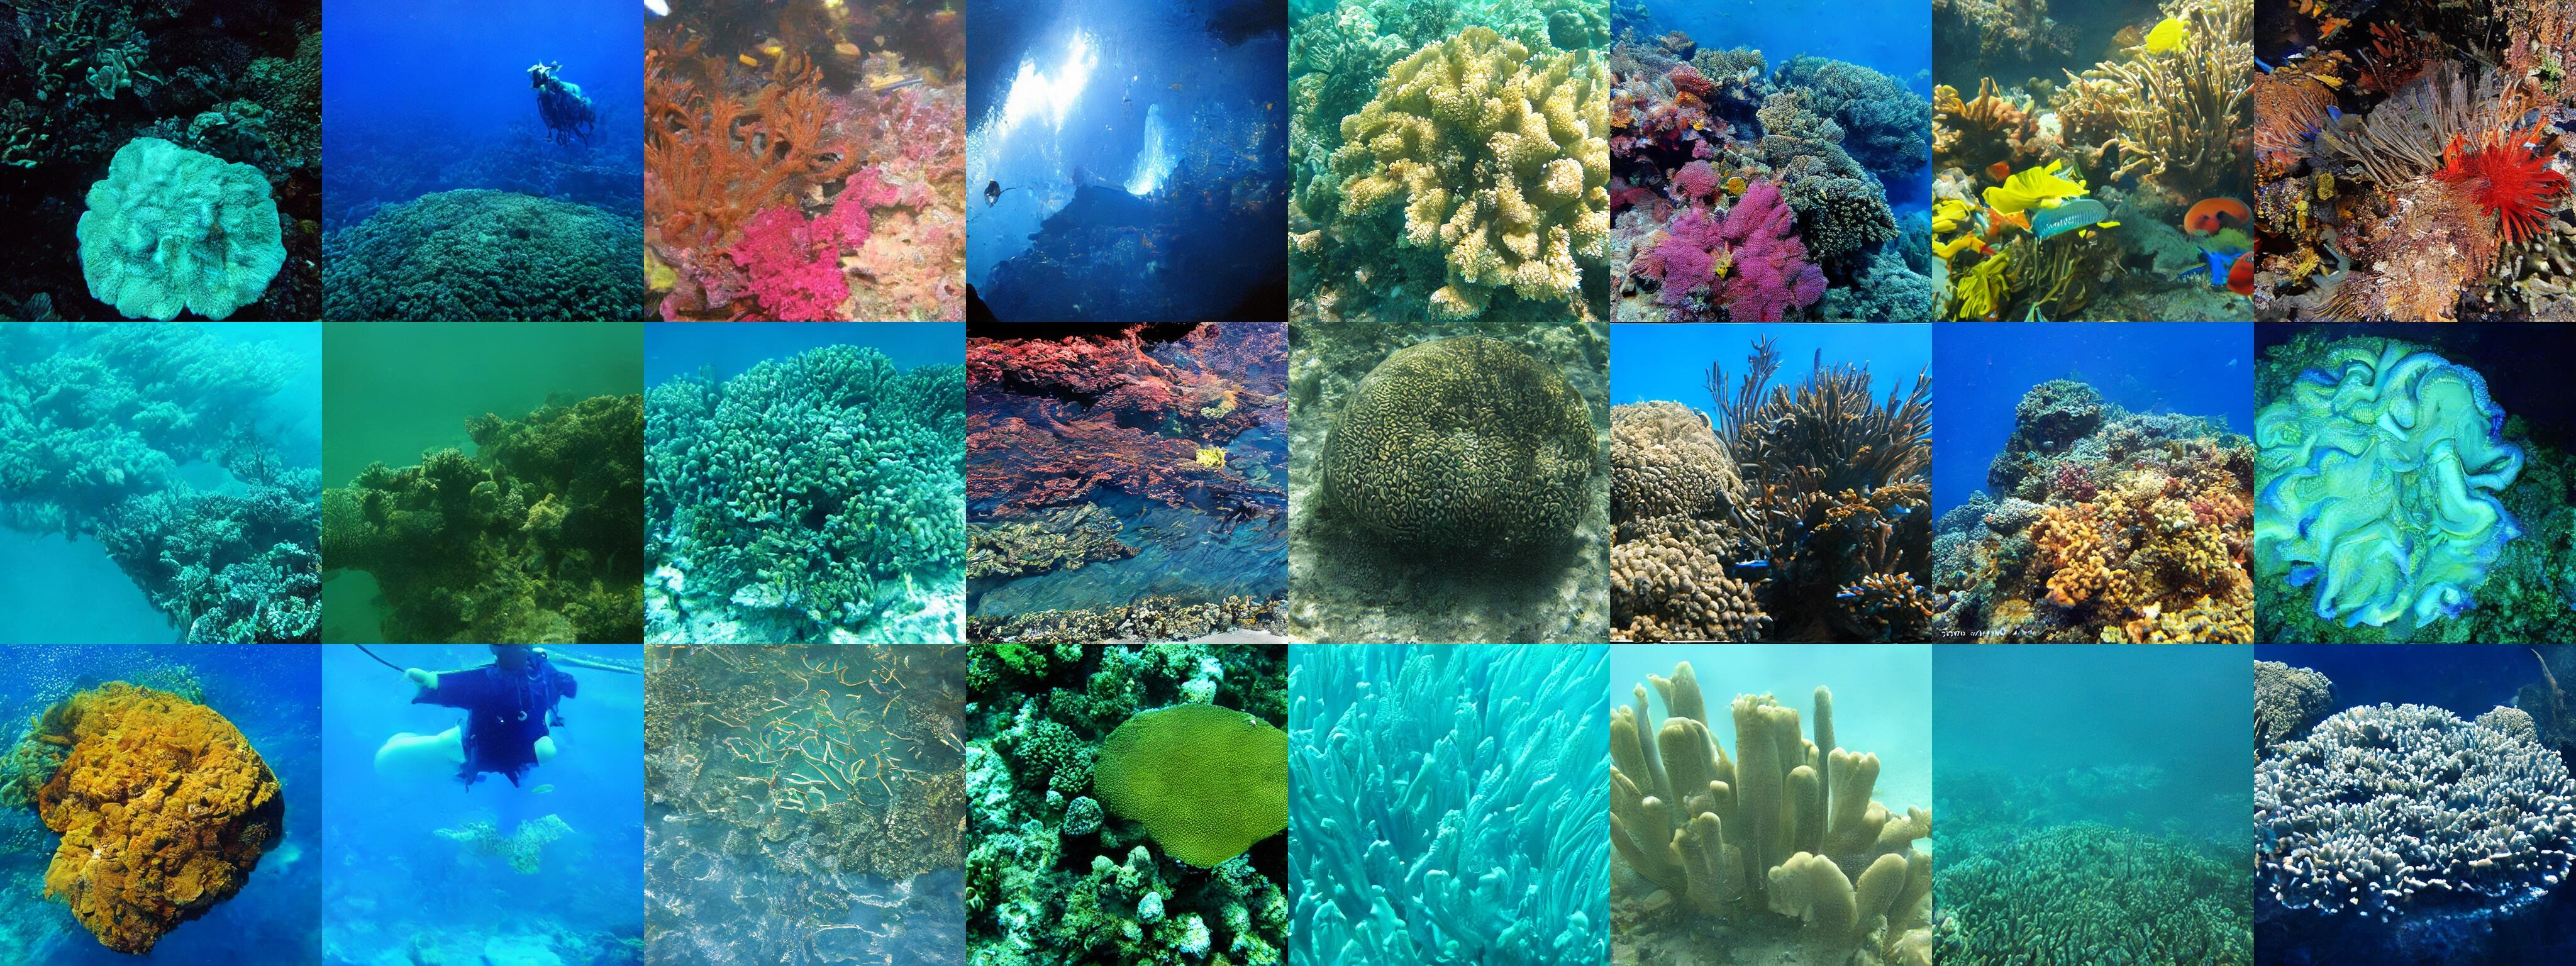
\includegraphics[width=\linewidth]{figures/samples-appendix-1step/973_batch.jpg}\\
	\end{minipage} \\

	\caption{\small{Uncurated 1-step samples generated by our sCD-XXL trained on ImageNet 512$\times$512.}
	\label{fig:appendix:samples-3-1step}}
\end{figure}



\begin{figure}[H]
 	\begin{minipage}{0.05\linewidth}
         \rotatebox{90}{\small{Class 417 (balloon), guidance 1.9}}
		\centering
	\end{minipage}
	\begin{minipage}{0.93\linewidth}
		\centering
        
\includegraphics[width=\linewidth]{figures/samples-appendix/417_batch.jpg}\\
	\end{minipage} \\

        \vspace{.2cm}
 	\begin{minipage}{0.05\linewidth}
         \rotatebox{90}{\small{Class 425 (barn), guidance 1.9}}
		\centering
	\end{minipage}
	\begin{minipage}{0.93\linewidth}
		\centering
        
\includegraphics[width=\linewidth]{figures/samples-appendix/425_batch.jpg}\\
	\end{minipage} \\

                \vspace{.2cm}
 	\begin{minipage}{0.05\linewidth}
         \rotatebox{90}{\small{Class 933 (cheeseburger), guidance 1.9}}
		\centering
	\end{minipage}
	\begin{minipage}{0.93\linewidth}
		\centering
        
\includegraphics[width=\linewidth]{figures/samples-appendix/933_batch.jpg}\\
	\end{minipage} \\
                \vspace{.2cm}
 	\begin{minipage}{0.05\linewidth}
         \rotatebox{90}{\small{Class 973 (coral reef), guidance 1.9}}
		\centering
	\end{minipage}
	\begin{minipage}{0.93\linewidth}
		\centering
        
\includegraphics[width=\linewidth]{figures/samples-appendix/973_batch.jpg}\\
	\end{minipage} \\

	\caption{\small{Uncurated 2-step samples generated by our sCD-XXL trained on ImageNet 512$\times$512.}
	\label{fig:appendix:samples-3}}
\end{figure}
